\documentclass[a4paper,12pt]{article}
\usepackage[utf8]{inputenc}
\usepackage[T1]{fontenc}
\usepackage[italian]{babel}
\usepackage{amsmath}
\usepackage{geometry}
\geometry{margin=2.5cm}
\usepackage{amsmath}
\usepackage{float}
\usepackage{graphicx}
\graphicspath{{src/}}
% consente i page‐break negli align
\allowdisplaybreaks
\title{Esercitazione Plant Layout\\Versione 1.0 a.a. 2024/2025}
\author{%
  Michele Mazza
    \and
  Gabriele Rossi
   \and
  Tommaso Veldhuyzen
}
\date{}

\begin{document}
\maketitle

Si richiede di progettare il layout di un nuovo stabilimento produttivo. 
La movimentazione viene effettuata mediante l’ausilio di carrelli elevatori a forche frontali (chiamati ``muletti'') e transpallet manuali.

\section{Dimensionamento dei reparti 7, 9 e 10}
Per dimensionare i reparti 7 (FMS taglio laser lamiera), 9 (tornitura) e 10 (centro di lavoro acciaio) si considerano i cicli di lavorazione di due prodotti caratteristici (Prodotto XXYa e Prodotto XXYb), rappresentativi di due famiglie (Famiglia 1 e Famiglia 2). 
Si desidera calcolare il numero minimo di risorse da dedicare a ciascuno di questi reparti.
\subsection{Dimensionamento teorico dei reparti}
Il tipo di layout adottato è il layout per reparti, in cui le macchine sono raggruppate in base alla loro funzione, abbiamo dunque adottato un approccio di dimensionamento statico, in cui si calcola il numero di macchine necessarie per soddisfare la domanda di produzione mensile dei prodotti XXYa e XXYb.
Per ciascun reparto, si calcola il tempo di lavorazione totale mensile, il tempo di lavorazione disponibile mensile e il numero di macchine necessarie, considerando le disponibilità di tempo e spazio.
Dopo aver calcolato il numero di macchine, si calcola l'area totale del reparto, moltiplicando lo spazio standard per il numero di macchine.
\subsubsection{Dati di input}
\begin{align*}
  &t_{i,j}  \left[\frac{\mathrm{min}}{\mathrm{pz}}\right], \text{Tempo unitario di lavorazione del Prodotto } i\in \left\{ \text{XXYa}, \text{XXYb}\right\} \text{nel reparto j}  \\
  &Q_{i,j} \left[\frac{\mathrm{pz}}{\mathrm{mese}}\right], \text{Volume produttivo mensile del Prodotto i nel reparto j}  \\
  &G_{\text{disp},j} \left[\frac{\mathrm{gg}}{\mathrm{mese}}\right], \text{Giorni lavorativi mensili disponibili nel reparto j} \\
  &R_{\text{disp},j}\left[\frac{\mathrm{turni}}{\mathrm{gg}}\right], \text{Turni di lavoro giornalieri nel reparto j}  \\
  &H_{\text{disp},j}\left[\frac{\mathrm{h}}{\mathrm{turno}}\right], \text{Ore lavorative giornaliere nel reparto j}  \\
  &\text{A}_j = \text{Availability del reparto j} \\
  &n_j = \left\lceil  \frac{T_{\text{tot},j}}{T_{\text{disp},j}}\right\rceil \left[\text{macchine}\right], \text{numero di macchine nel reparto j} \\
  & A_{u_j} \left[\frac{\mathrm{m}^2}{\text{macchina}}\right] = \text{Spazio standard del reparto j}  \\
\end{align*}
\subsubsection{Formule di calcolo}
\begin{align*}
  &T_{\text{tot},j} = \sum_{i} t_{i,j} \times Q_{i,j} \left[\frac{\mathrm{h}}{\mathrm{mese}}\right], \text{Tempo di lavorazione disponibile mensile nel reparto j}  \\
  &T_{\text{disp},j} = G_{\text{disp},j} \times R_{\text{disp},j} \times H_{\text{disp},j} \times A_j  \left[\frac{\mathrm{h}}{\mathrm{mese}}\right], \text{Tempo di lavorazione disponibile mensile nel reparto j} \\
  &n_j = \left\lceil  \frac{T_{\text{tot},j}}{T_{\text{disp},j}}\right\rceil \left[\text{macchine}\right], \text{numero di macchine nel reparto j} \\
  &A_j = A_{u_j} \times n_j \left[\mathrm{m}^2\right], \text{Area del reparto j}  \\
\end{align*}

\subsection{Reparto 7: FMS taglio laser lamiera}
{\small
\begin{align*}
 &t_{a,7}\,\bigl[\tfrac{\min}{\mathrm{pz}}\bigr]\times Q_{a,7}\,\bigl[\tfrac{\mathrm{pz}}{\mathrm{mese}}\bigr]
 =11.9\times412=4902.8\;\bigl[\tfrac{\min}{\mathrm{mese}}\bigr],\\
 &t_{b,7}\,\bigl[\tfrac{\min}{\mathrm{pz}}\bigr]\times Q_{b,7}\,\bigl[\tfrac{\mathrm{pz}}{\mathrm{mese}}\bigr]
 =26.0\times300=7800\;\bigl[\tfrac{\min}{\mathrm{mese}}\bigr],\\
 &T_{\mathrm{tot},7}^{[\min]}=4902.8+7800=12702.8\;\bigl[\tfrac{\min}{\mathrm{mese}}\bigr],\\
 &T_{\mathrm{tot},7}^{[\mathrm{h}]}=\frac{12702.8}{60}=211.713\;\bigl[\tfrac{\mathrm{h}}{\mathrm{mese}}\bigr],\\
 &T_{\mathrm{disp},7}
 =G_{\mathrm{disp},7}\times R_{\mathrm{disp},7}\times H_{\mathrm{disp},7}\times\text{A}_7
 =21\times2\times8\times0.95
 =319.2\;\bigl[\tfrac{\mathrm{h}}{\mathrm{mese}}\bigr],\\
 &n_{7}=\left\lceil\frac{T_{\mathrm{tot},7}^{[\mathrm{h}]}}{T_{\mathrm{disp},7}}\right\rceil
 =\bigl\lceil\tfrac{211.713}{319.2}\bigr\rceil=1,\\
 &A_{7}=A_{u,7}\times N_{7}=500\times1=500\;\bigl[\mathrm{m}^2\bigr].
\end{align*}
}

\subsection{Reparto 9: Tornitura}
{\small
\begin{align*}
 &t_{a,9}\,\bigl[\tfrac{\min}{\mathrm{pz}}\bigr]\times Q_{a,9}\,\bigl[\tfrac{\mathrm{pz}}{\mathrm{mese}}\bigr]
 =59.3\times412=24431.6\;\bigl[\tfrac{\min}{\mathrm{mese}}\bigr],\\
 &t_{b,9}\,\bigl[\tfrac{\min}{\mathrm{pz}}\bigr]\times Q_{b,9}\,\bigl[\tfrac{\mathrm{pz}}{\mathrm{mese}}\bigr]
 =0\times300=0\;\bigl[\tfrac{\min}{\mathrm{mese}}\bigr],\\
 &T_{\mathrm{tot},9}^{[\min]}=24431.6\;\bigl[\tfrac{\min}{\mathrm{mese}}\bigr],\quad
 T_{\mathrm{tot},9}^{[\mathrm{h}]}=\tfrac{24431.6}{60}=407.193\;\bigl[\tfrac{\mathrm{h}}{\mathrm{mese}}\bigr],\\
 &T_{\mathrm{disp},9}
 =G_{\mathrm{disp},9}\times R_{\mathrm{disp},9}\times H_{\mathrm{disp},9}\times\text{A}_9
 =21\times1\times8\times0.99
 =166.32\;\bigl[\tfrac{\mathrm{h}}{\mathrm{mese}}\bigr],\\
 &n_{9}=\left\lceil\frac{407.193}{166.32}\right\rceil
 =\bigl\lceil2.45\bigr\rceil=3,\\
 &A_{9}=A_{u,9}\times N_{9}=300\times3=900\;\bigl[\mathrm{m}^2\bigr].
\end{align*}
}

\subsection{Reparto 10: Centro di lavoro acciaio}
{\small
\begin{align*}
 &t_{a,10}\,\bigl[\tfrac{\min}{\mathrm{pz}}\bigr]\times Q_{a,10}\,\bigl[\tfrac{\mathrm{pz}}{\mathrm{mese}}\bigr]
 =27.8\times412=11453.6\;\bigl[\tfrac{\min}{\mathrm{mese}}\bigr],\\
 &t_{b,10}\,\bigl[\tfrac{\min}{\mathrm{pz}}\bigr]\times Q_{b,10}\,\bigl[\tfrac{\mathrm{pz}}{\mathrm{mese}}\bigr]
 =33.0\times300=9900\;\bigl[\tfrac{\min}{\mathrm{mese}}\bigr],\\
 &T_{\mathrm{tot},10}^{[\min]}=11453.6+9900=21353.6\;\bigl[\tfrac{\min}{\mathrm{mese}}\bigr],\\
 &T_{\mathrm{tot},10}^{[\mathrm{h}]}=\tfrac{21353.6}{60}=355.893\;\bigl[\tfrac{\mathrm{h}}{\mathrm{mese}}\bigr],\\
 &T_{\mathrm{disp},10}
 =G_{\mathrm{disp},10}\times R_{\mathrm{disp},10}\times H_{\mathrm{disp},10}\times\text{A}_10
 =21\times3\times8\times0.97
 =488.88\;\bigl[\tfrac{\mathrm{h}}{\mathrm{mese}}\bigr],\\
 &n_{10}=\left\lceil\frac{355.893}{488.88}\right\rceil
 =\bigl\lceil0.73\bigr\rceil=1,\\
 &A_{10}=A_{u,10}\times N_{10}=400\times1=400\;\bigl[\mathrm{m}^2\bigr].
\end{align*}
}


\section{Diagramma del flusso dei materiali}
Costruire il diagramma secondo la procedura SLP (es.\ CORELAP, ALDEP, TCR), giustificando le scelte e documentando i passi adottati.
\subsection{Piano di lavoro}
L'algoritmo scelto per la costruzione del layout è il TCR, per prima cosa abbiamo manipolato la matrice From-To presente in Tabella 3 riscrivendo la From-to dei flussi corrispondenti ad ogni CP, andando a riportare al di sopra della diagonale principale tutti i flussi totali, dopodichè abbiamo unito i flussi che riguardano i control point di scarico e di carico, ottenendo la matrice From-To riportata in Tabella 3.2, poi considerando che le attività di movimentazione e logistica sono effettuate nei due turni di lavoro giornalieri, ovvero indipendentemente dall'organizzazione del lavoro sulle macchine/reparti, si raddoppiano i valori di ciascu flusso per ottenere la matrice From-To riportata in Tabella 3.3.
\begin{figure}[H] % h = here, t = top, b = bottom, p = page
  \centering
  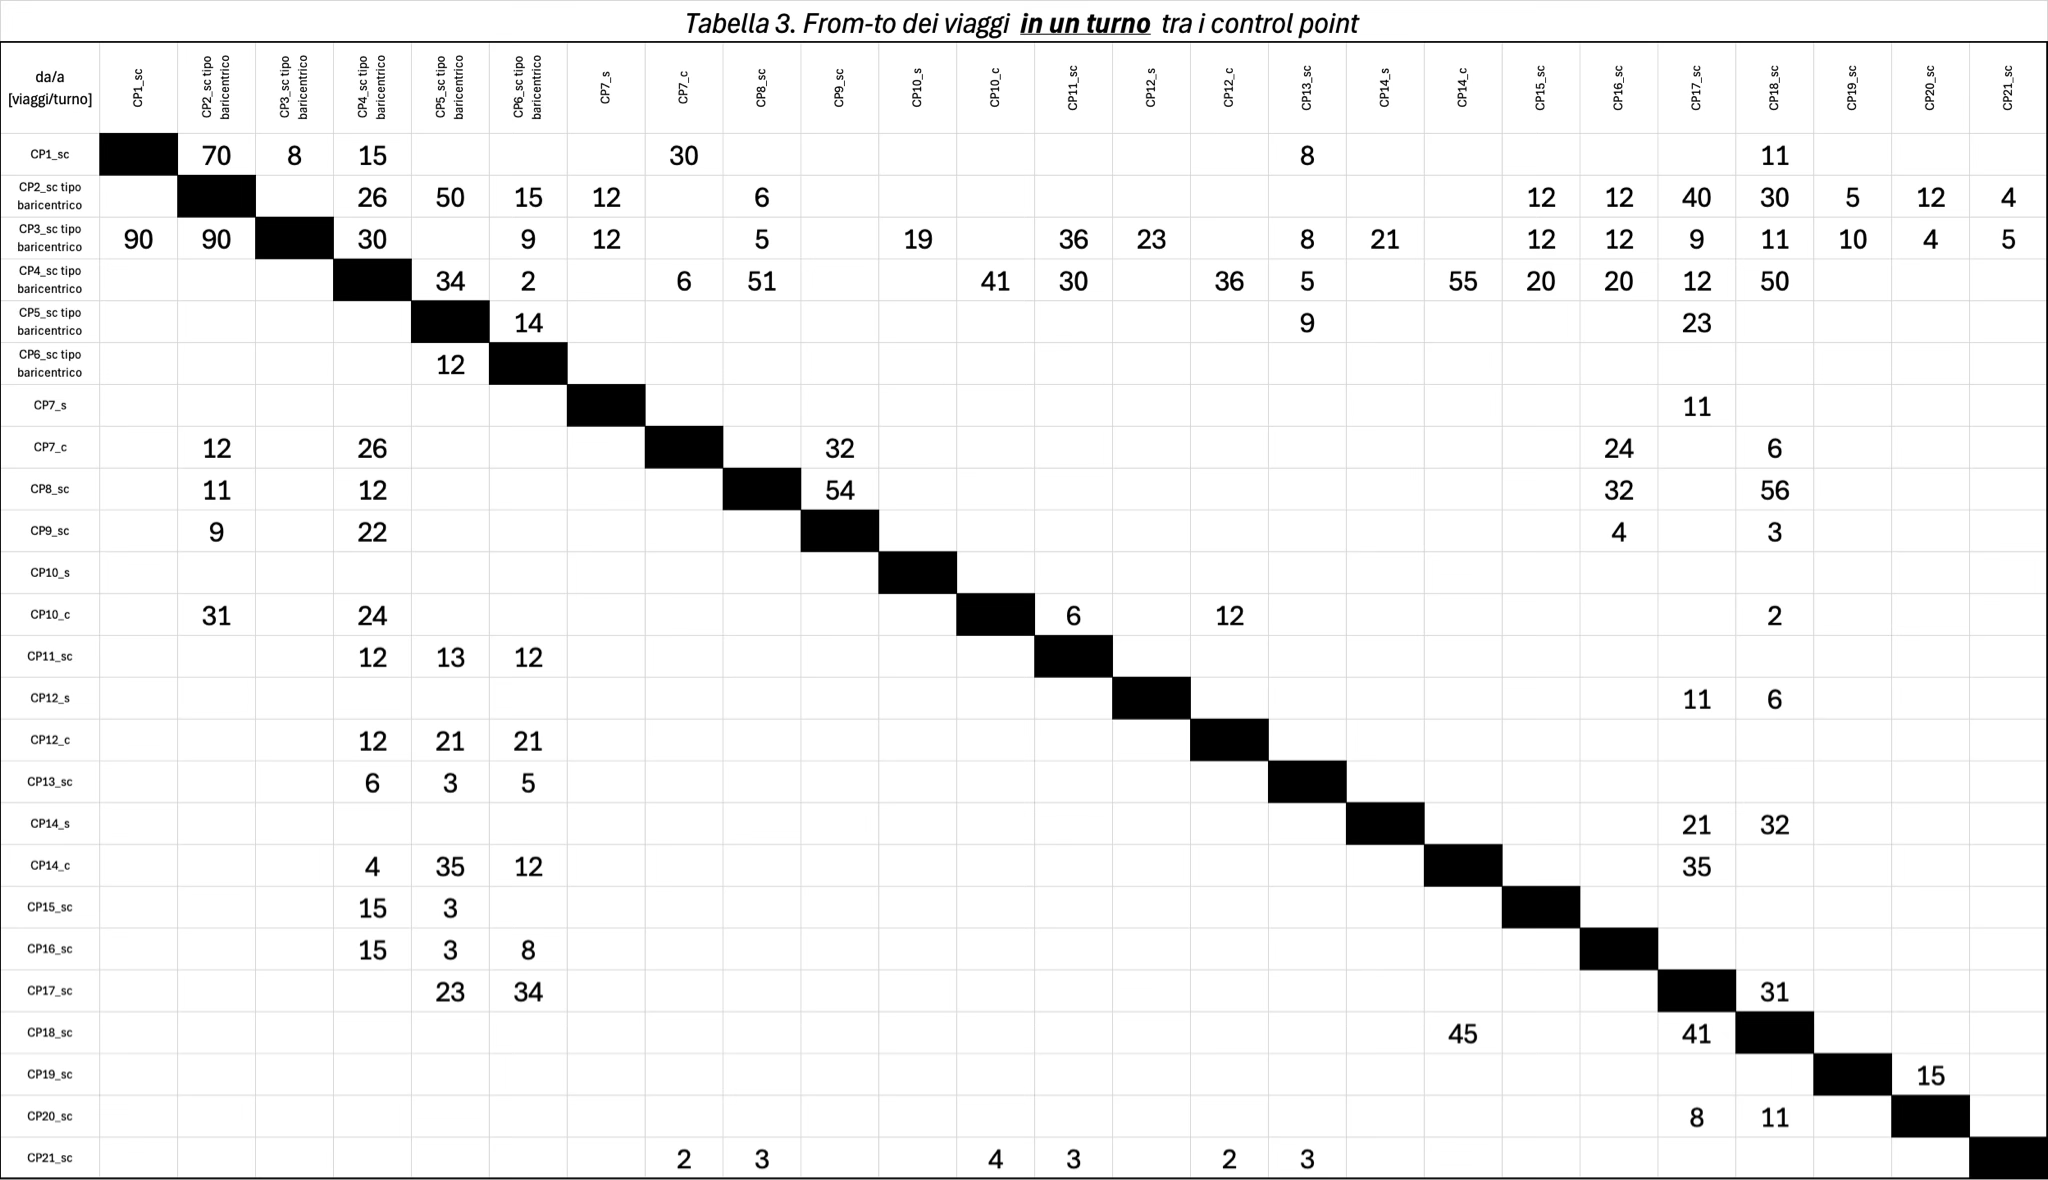
\includegraphics[width=0.4\textwidth]{Tabella 3.png}
  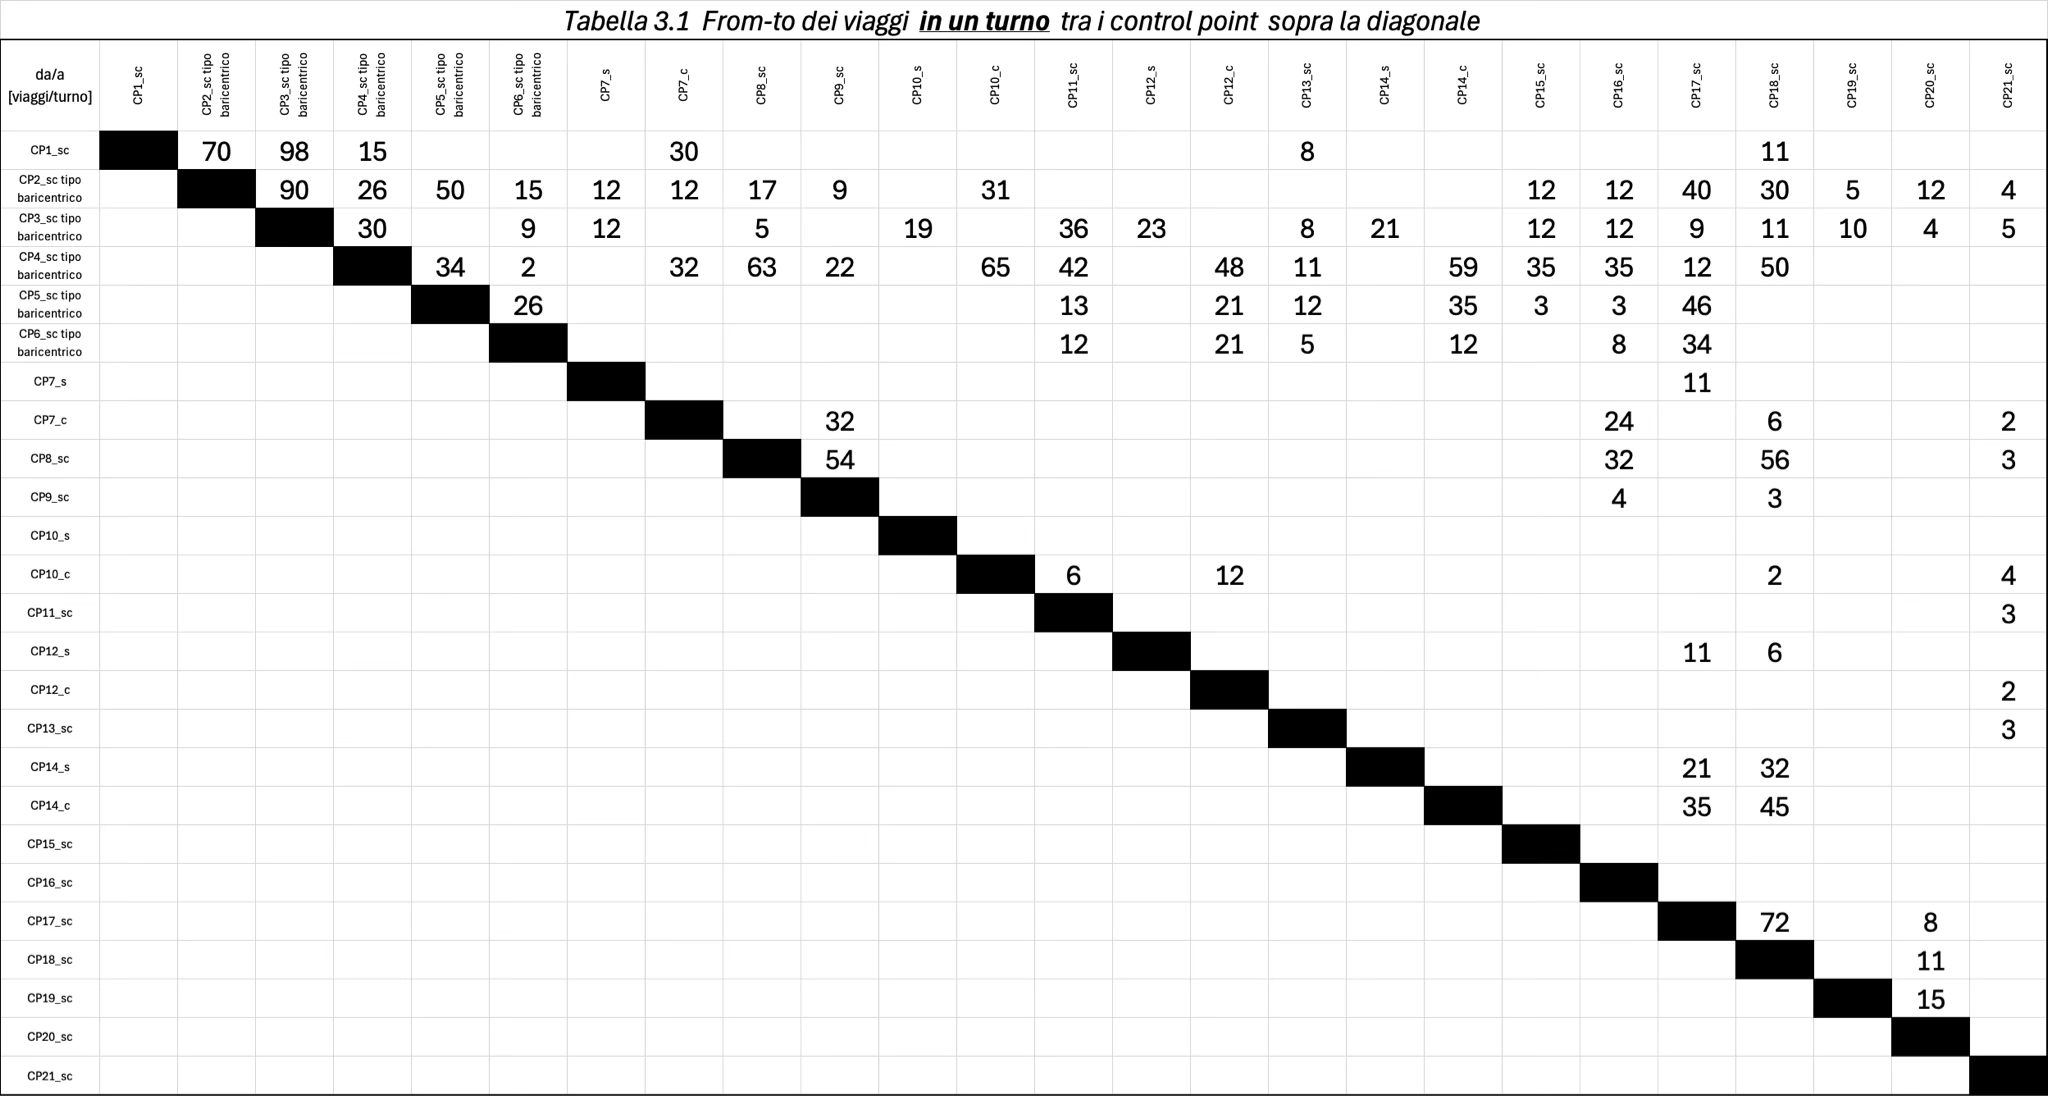
\includegraphics[width=0.4\textwidth]{Tabella3.1.png}
  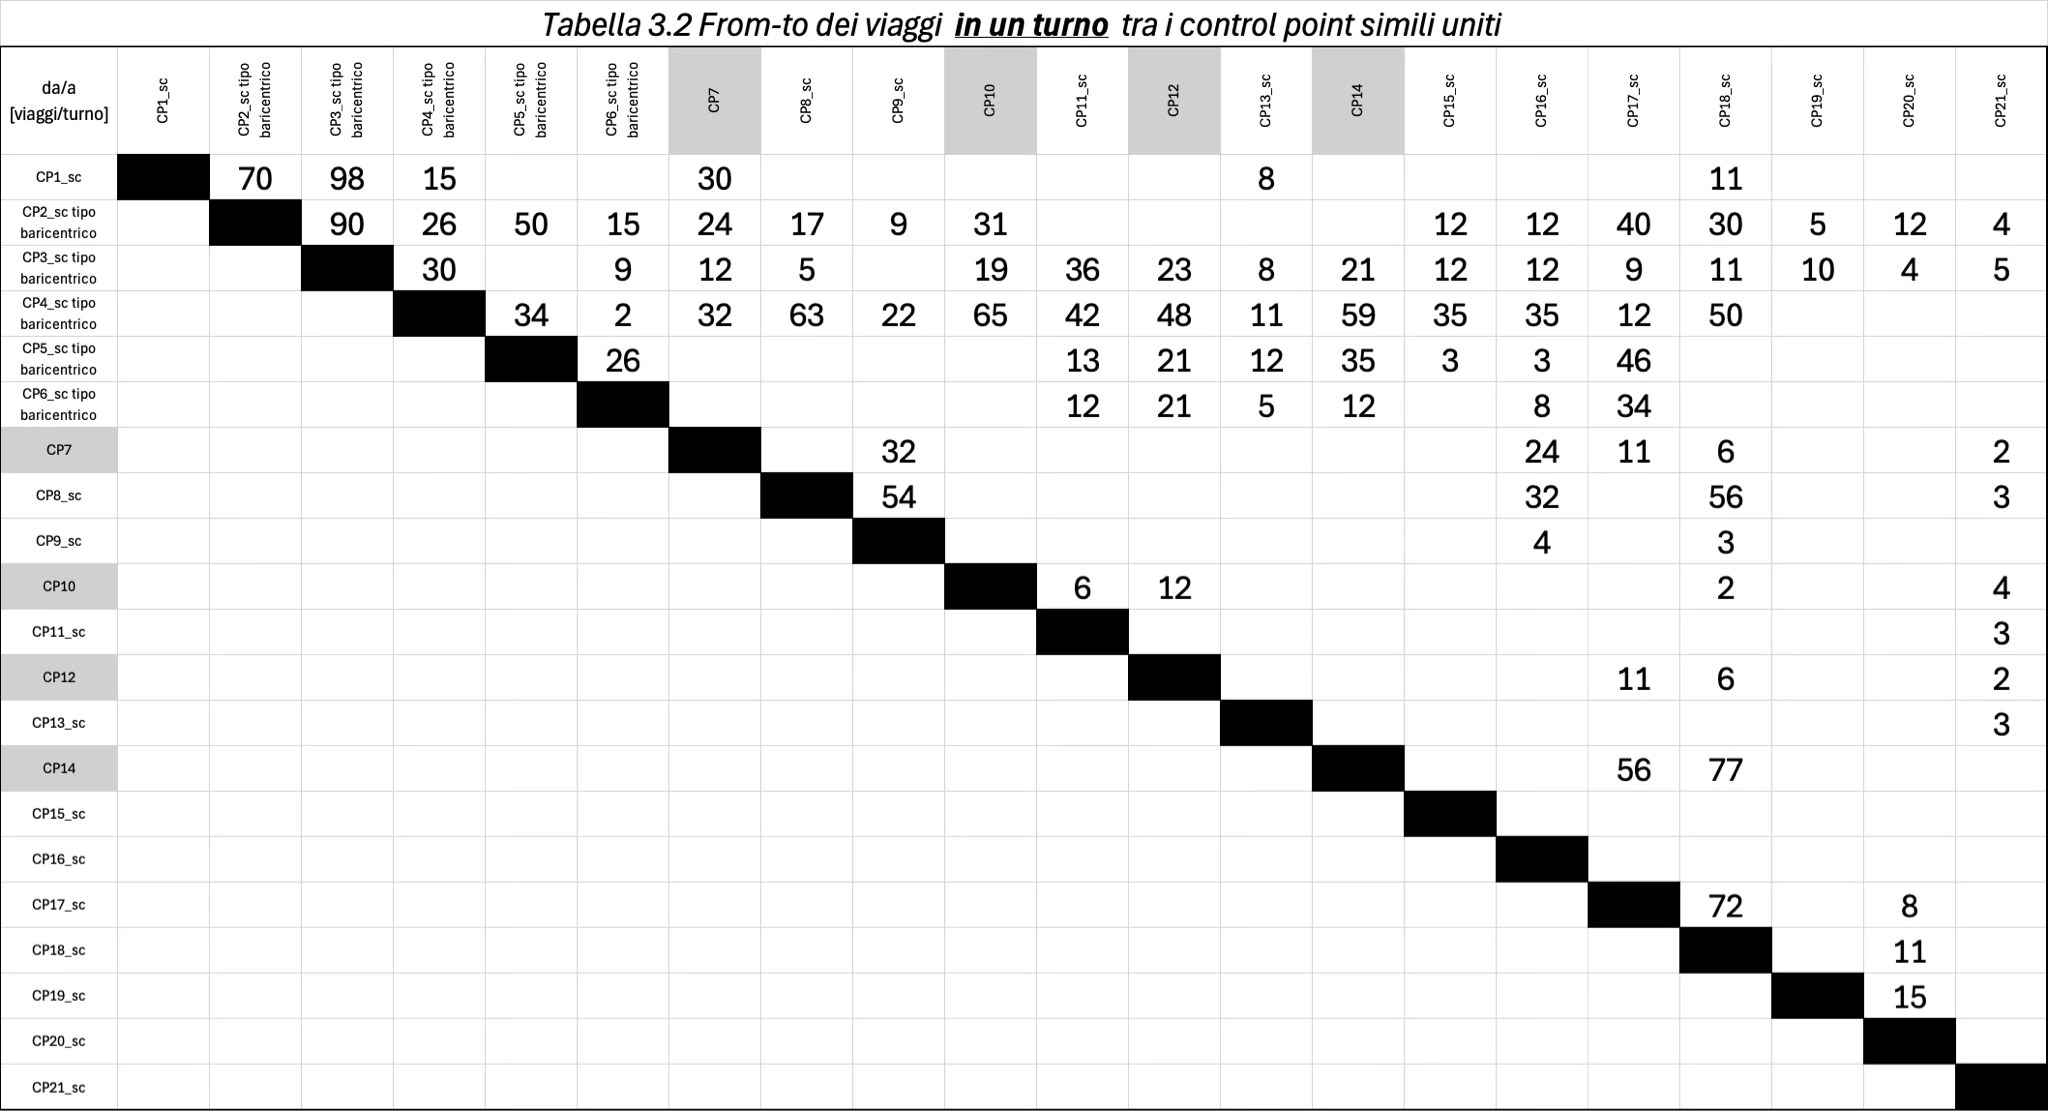
\includegraphics[width=0.4\textwidth]{Tabella3.2.png}
  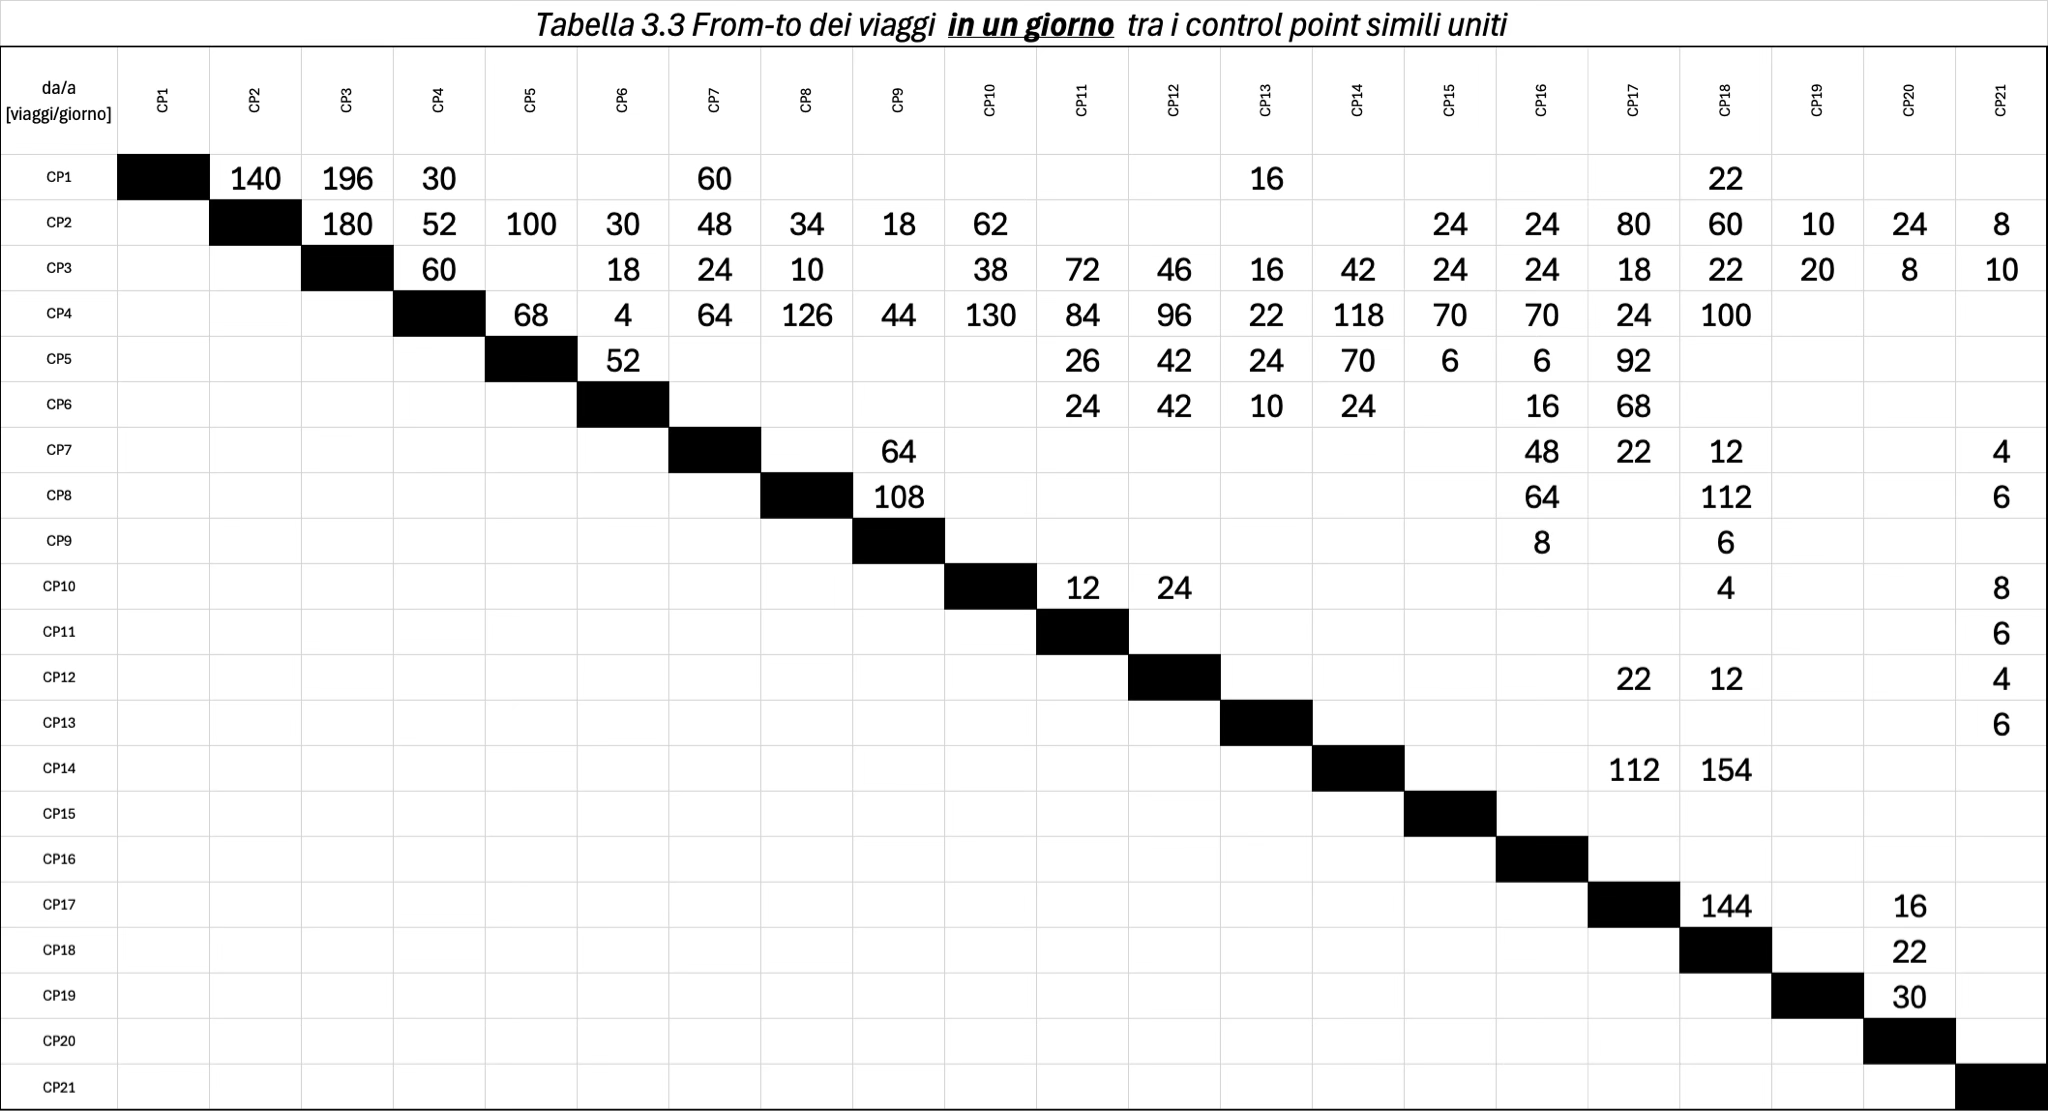
\includegraphics[width=0.4\textwidth]{Tabella3.3.png}
  \caption{Tabella 3: Matrici From-To}
  \label{fig:matrice-from-to 1}
\end{figure}

\subsection{Applicazione Algoritmo TCR}
Seguendo gli step della procedura del \textit{Systematic Layout Planning} abbiamo analizzato il flusso dei materiali e le relazioni tra i control point, per poi procedere con il ranking dei control point e la costruzione del layoutapplicando l'algoritmo TCR.
\subsubsection{Step 1: Ranking dei control point}
Abbiamo affrontanto la fase di ranking dei control point (CP) in tre fasi:
\begin{enumerate}
  \item Valutando i CP in base alla P-Matrix (Proximity Matrix) quantitativa dei flussi, fornita dal prof.
  \item Valutando i CP in base ad una R-Matrix (Relationship Matrix) la matrice qualitativa delle relazioni interfunzionali elaborata in base a dei codici motivazionali redatti e ragionati.
  \item La somma delle due matrici fornisce la S-Matrix un compromesso tra relazioni e flussi, che permette di calcolare il ranking dei CP.
\end{enumerate}
\subsubsection*{P-Matrix}
Nel caso della P-Matrix abbiamo i seguenti range di valori che associati alla matrice From-To riportata in Tabella 3.3 elaborano la P-Matrix.
\begin{figure}[H] 
  \centering
    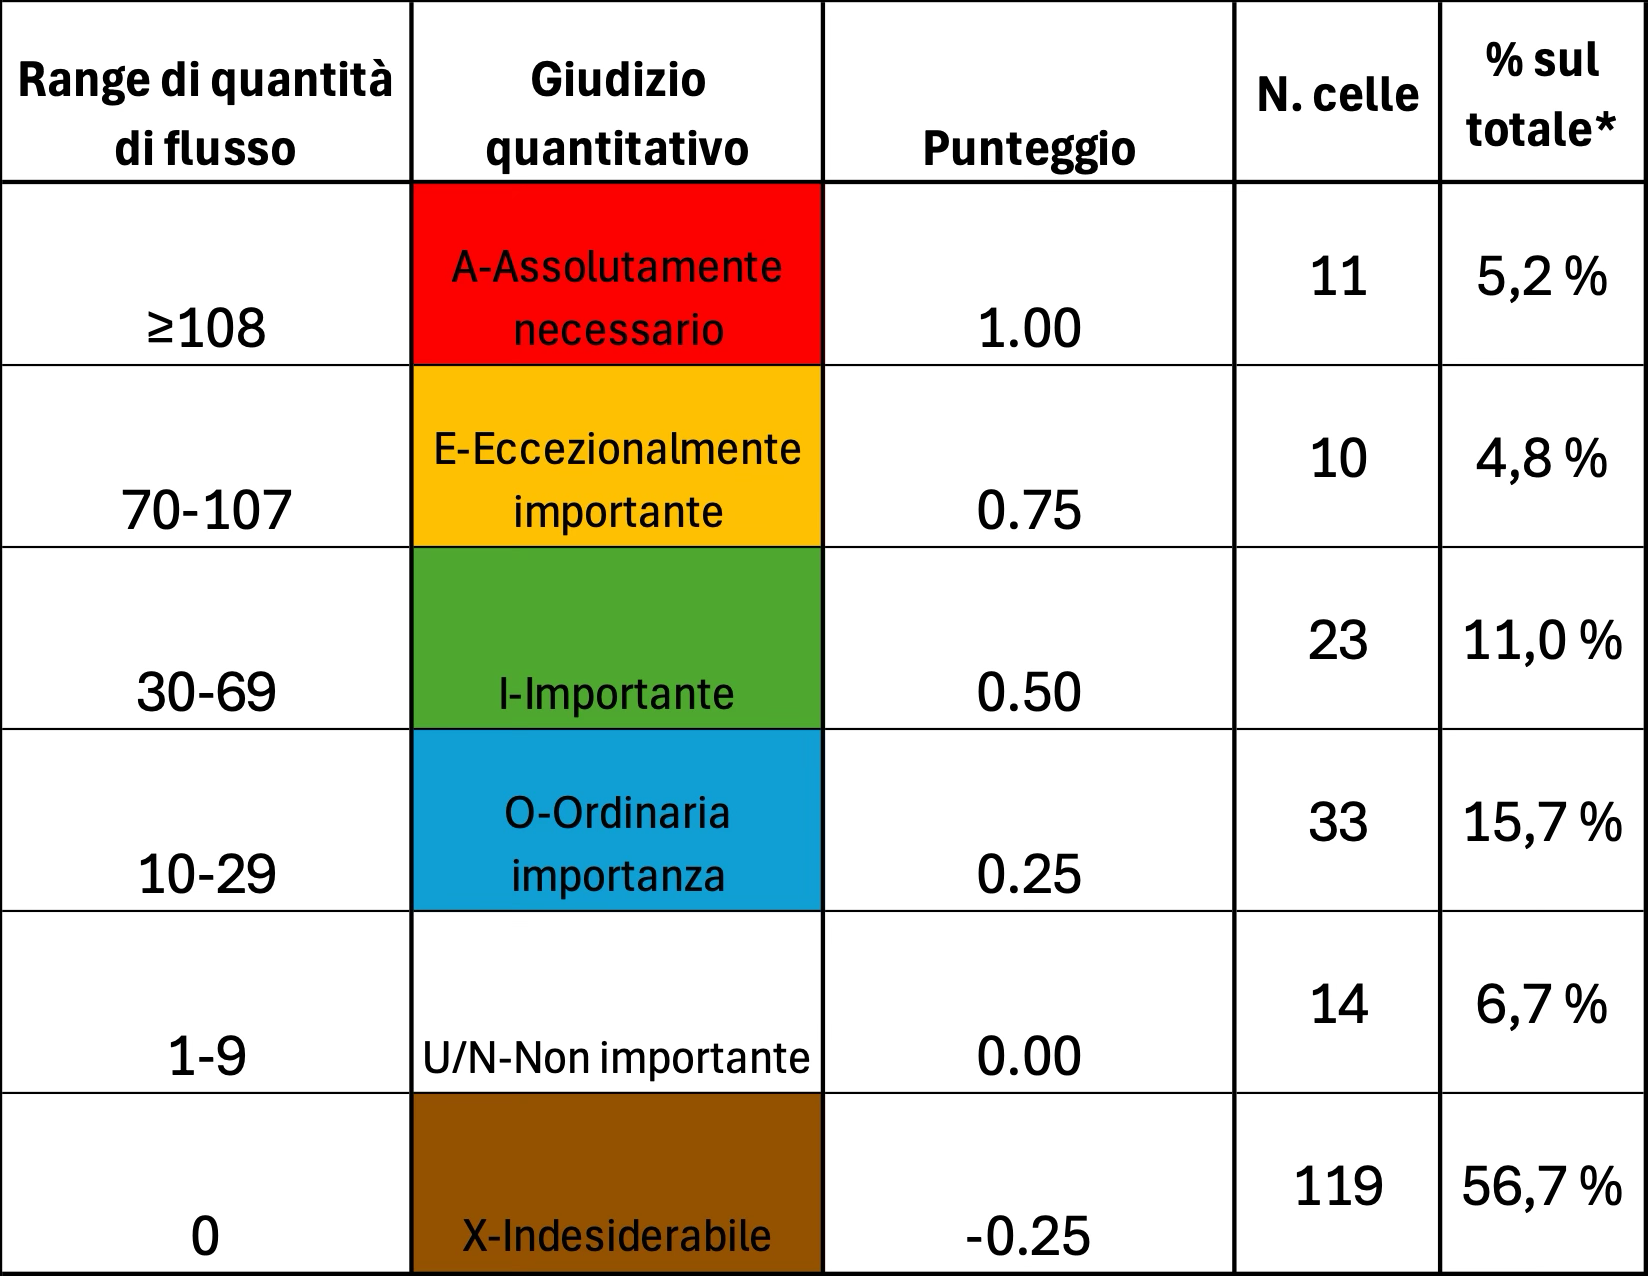
\includegraphics[width=0.5\textwidth]{P-Matrix Range.png}
  \caption{P-Matrix Range}
  \label{fig:P-Matrix Range}
\end{figure}
\begin{figure}[H]
  \centering
  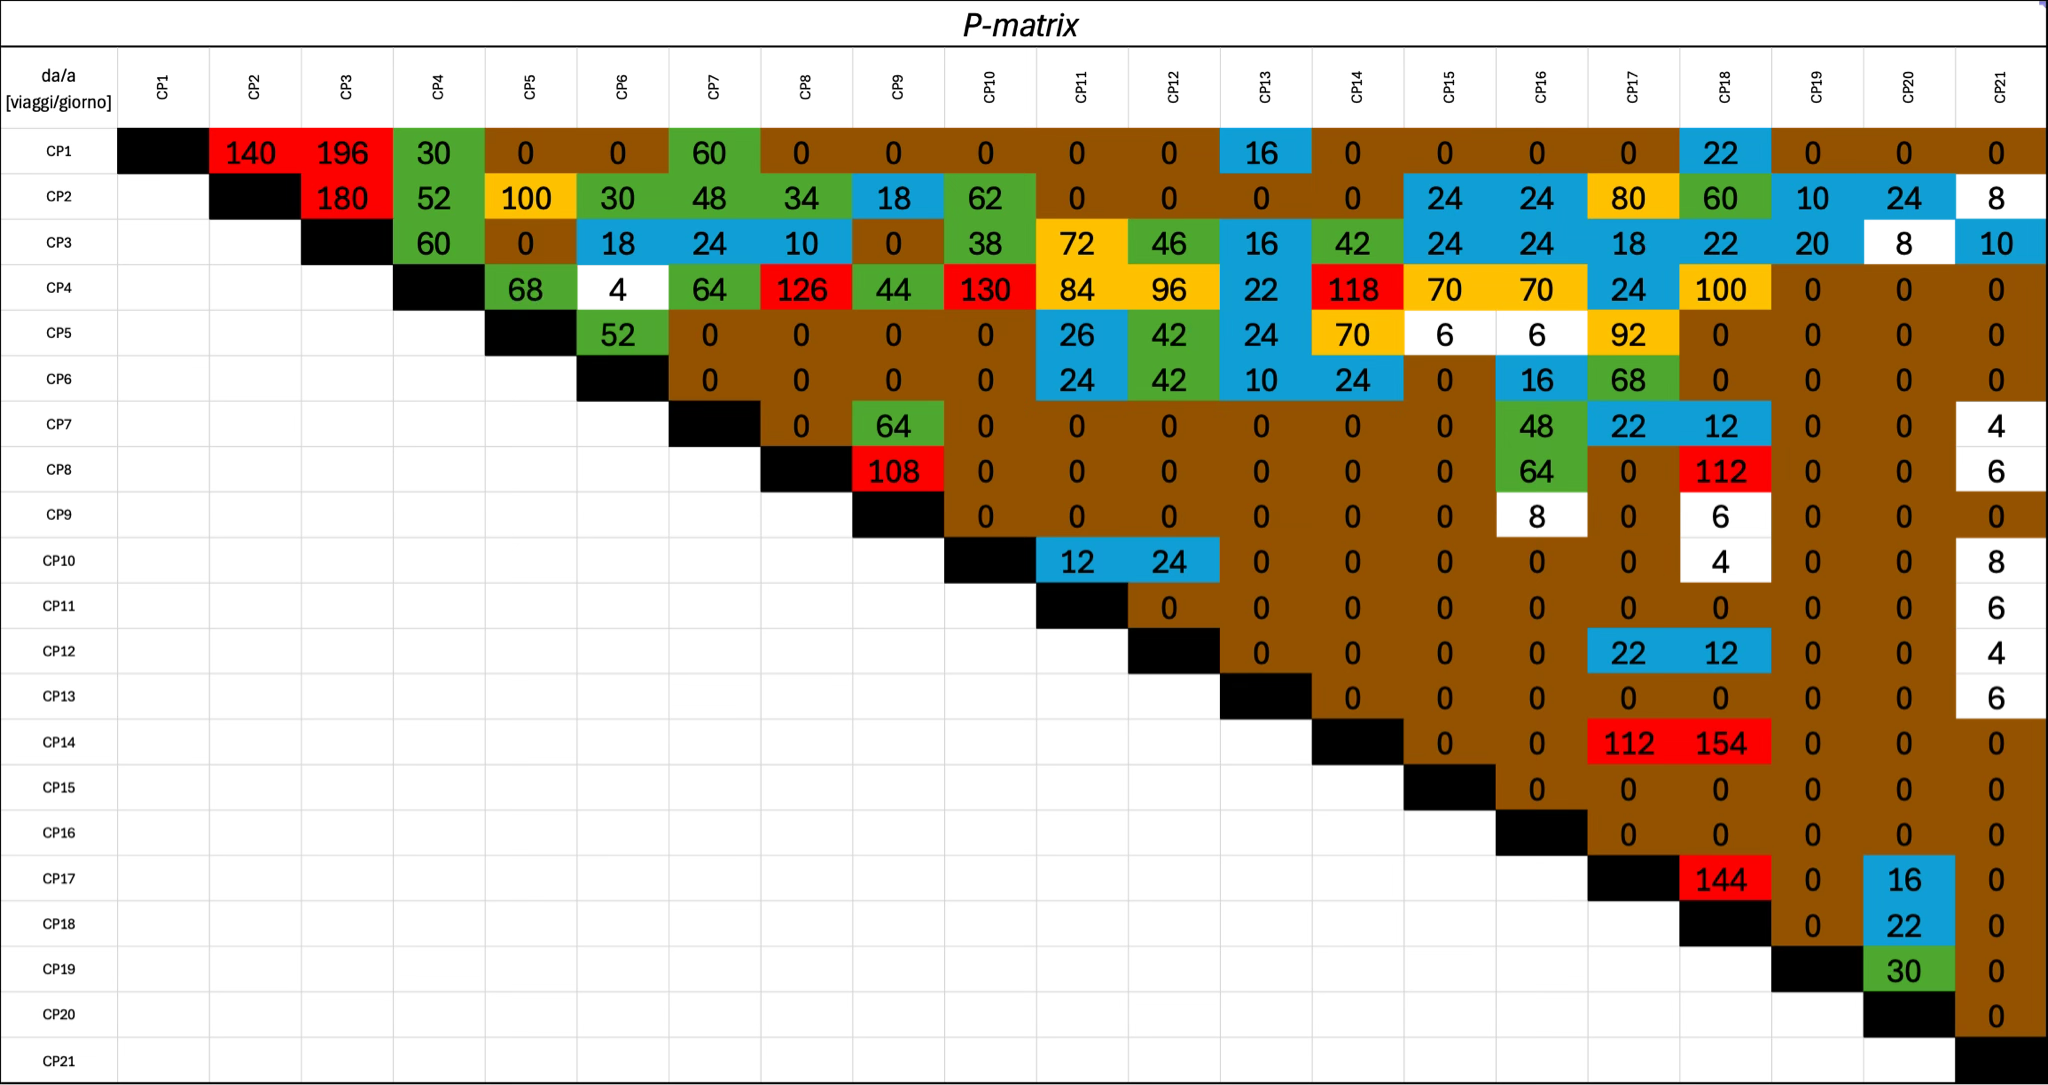
\includegraphics[width=0.7\textwidth]{P-Matrix Numbers.png}
  \caption{P-Matrix}
  \label{fig:P-Matrix Numbers}
\end{figure}
\begin{figure}[H]
  \centering
  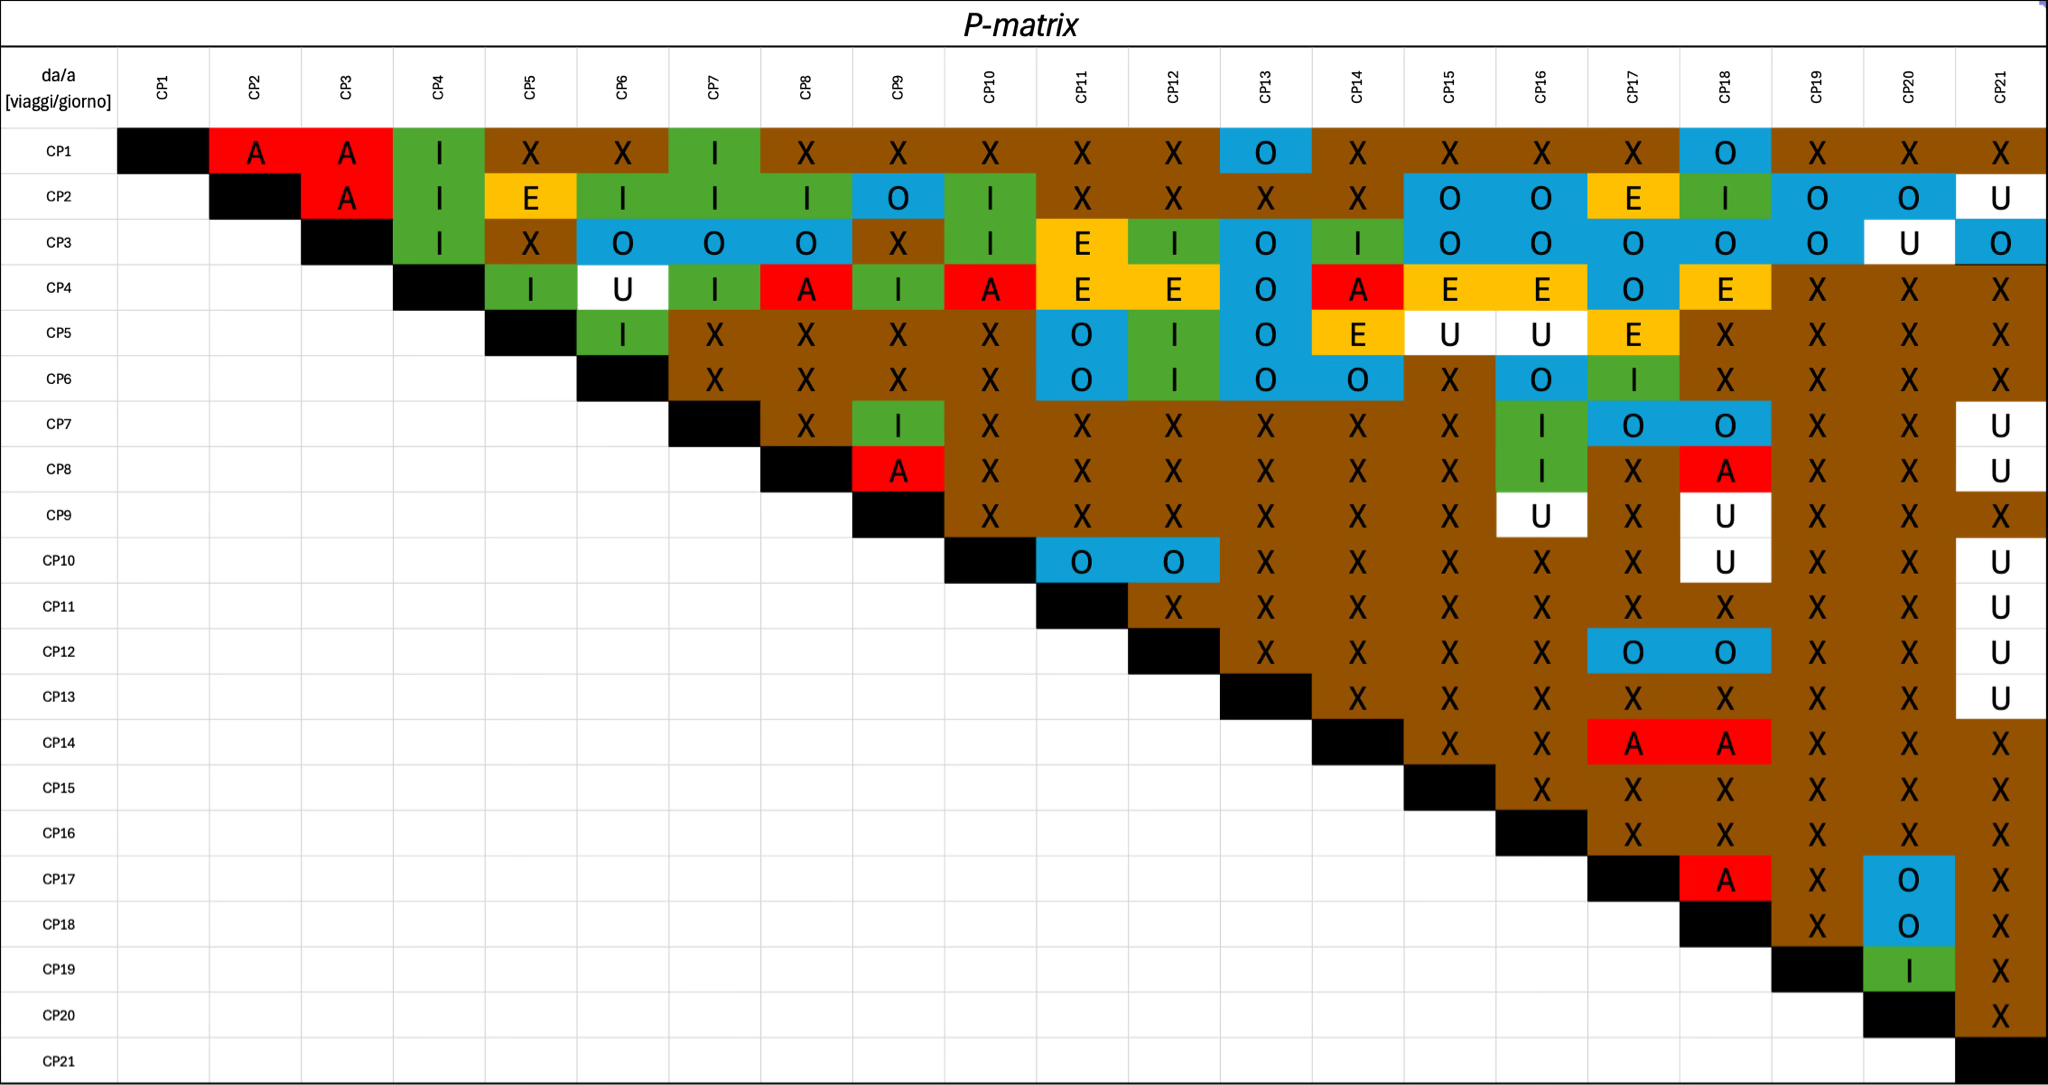
\includegraphics[width=0.7\textwidth]{P-Matrix Values.png}
  \caption{P-Matrix valori}
  \label{fig:P-Matrix Values}
\end{figure}
\subsubsection*{R-Matrix}
Nel caso della R-Matrix abbiamo i seguenti codici motivazionali che elaborano la matrice qualitativa delle relazioni interfunzionali:
\begin{figure}[H] 
  \centering
  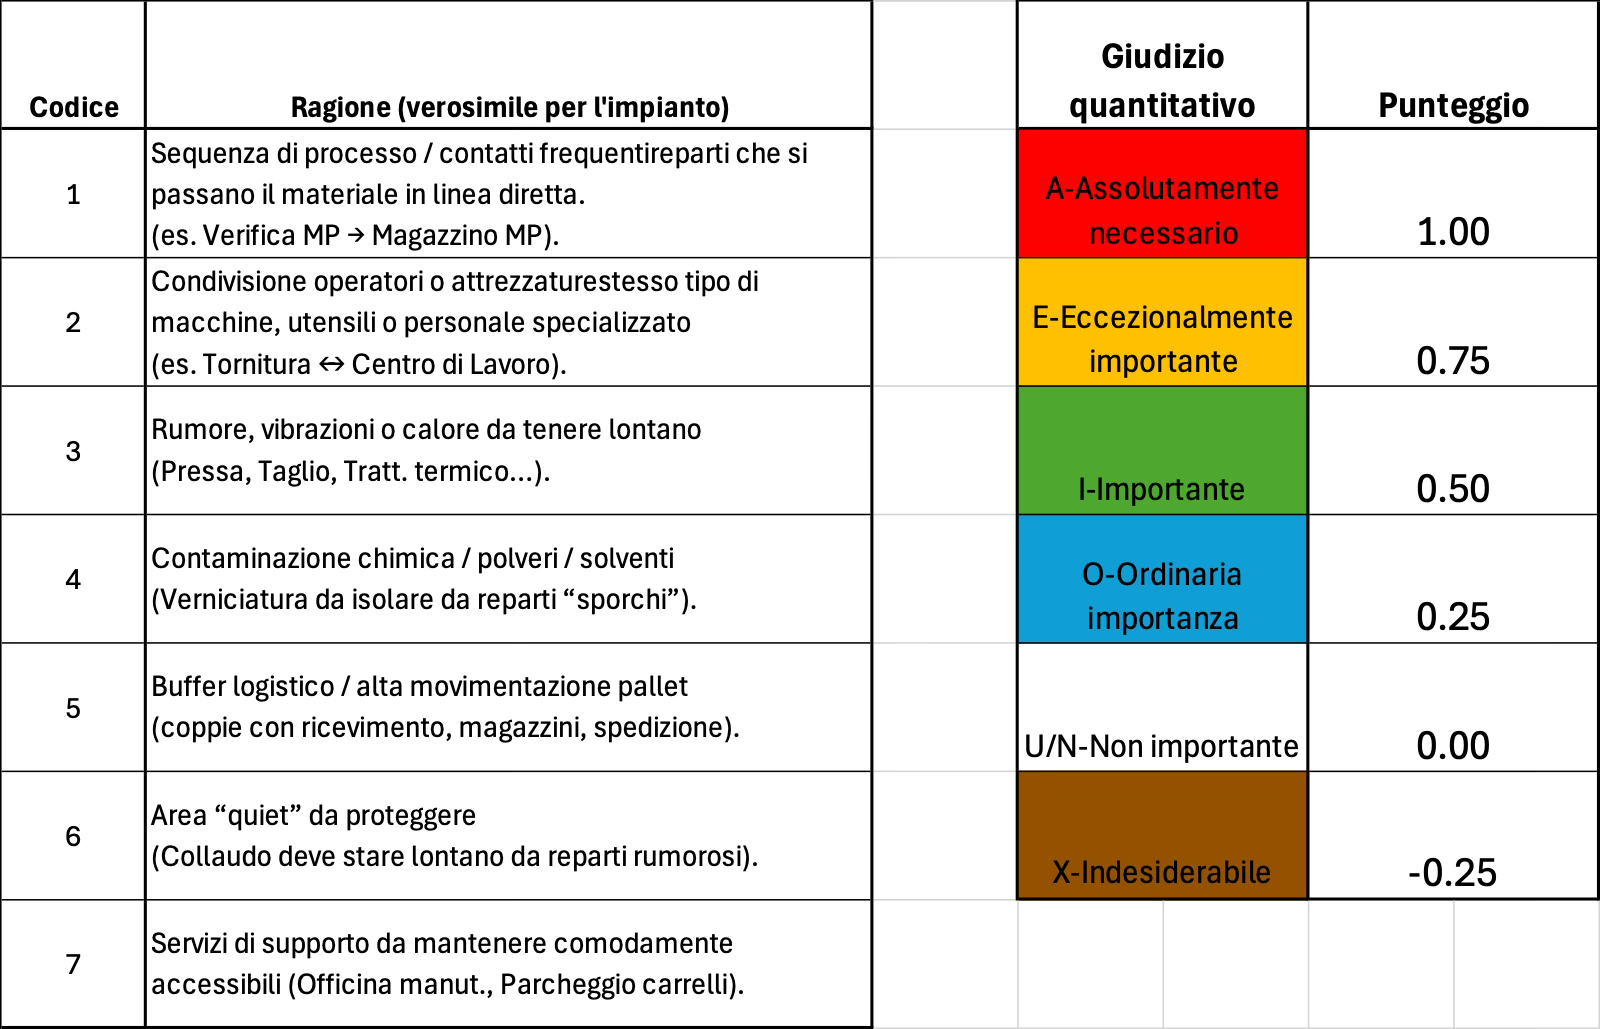
\includegraphics[width=0.5\textwidth]{R-Matrix Range.png}
  \caption{R-Matrix Range}
  \label{fig:R-Matrix Range}
\end{figure}
\begin{figure}[H]
  \centering
  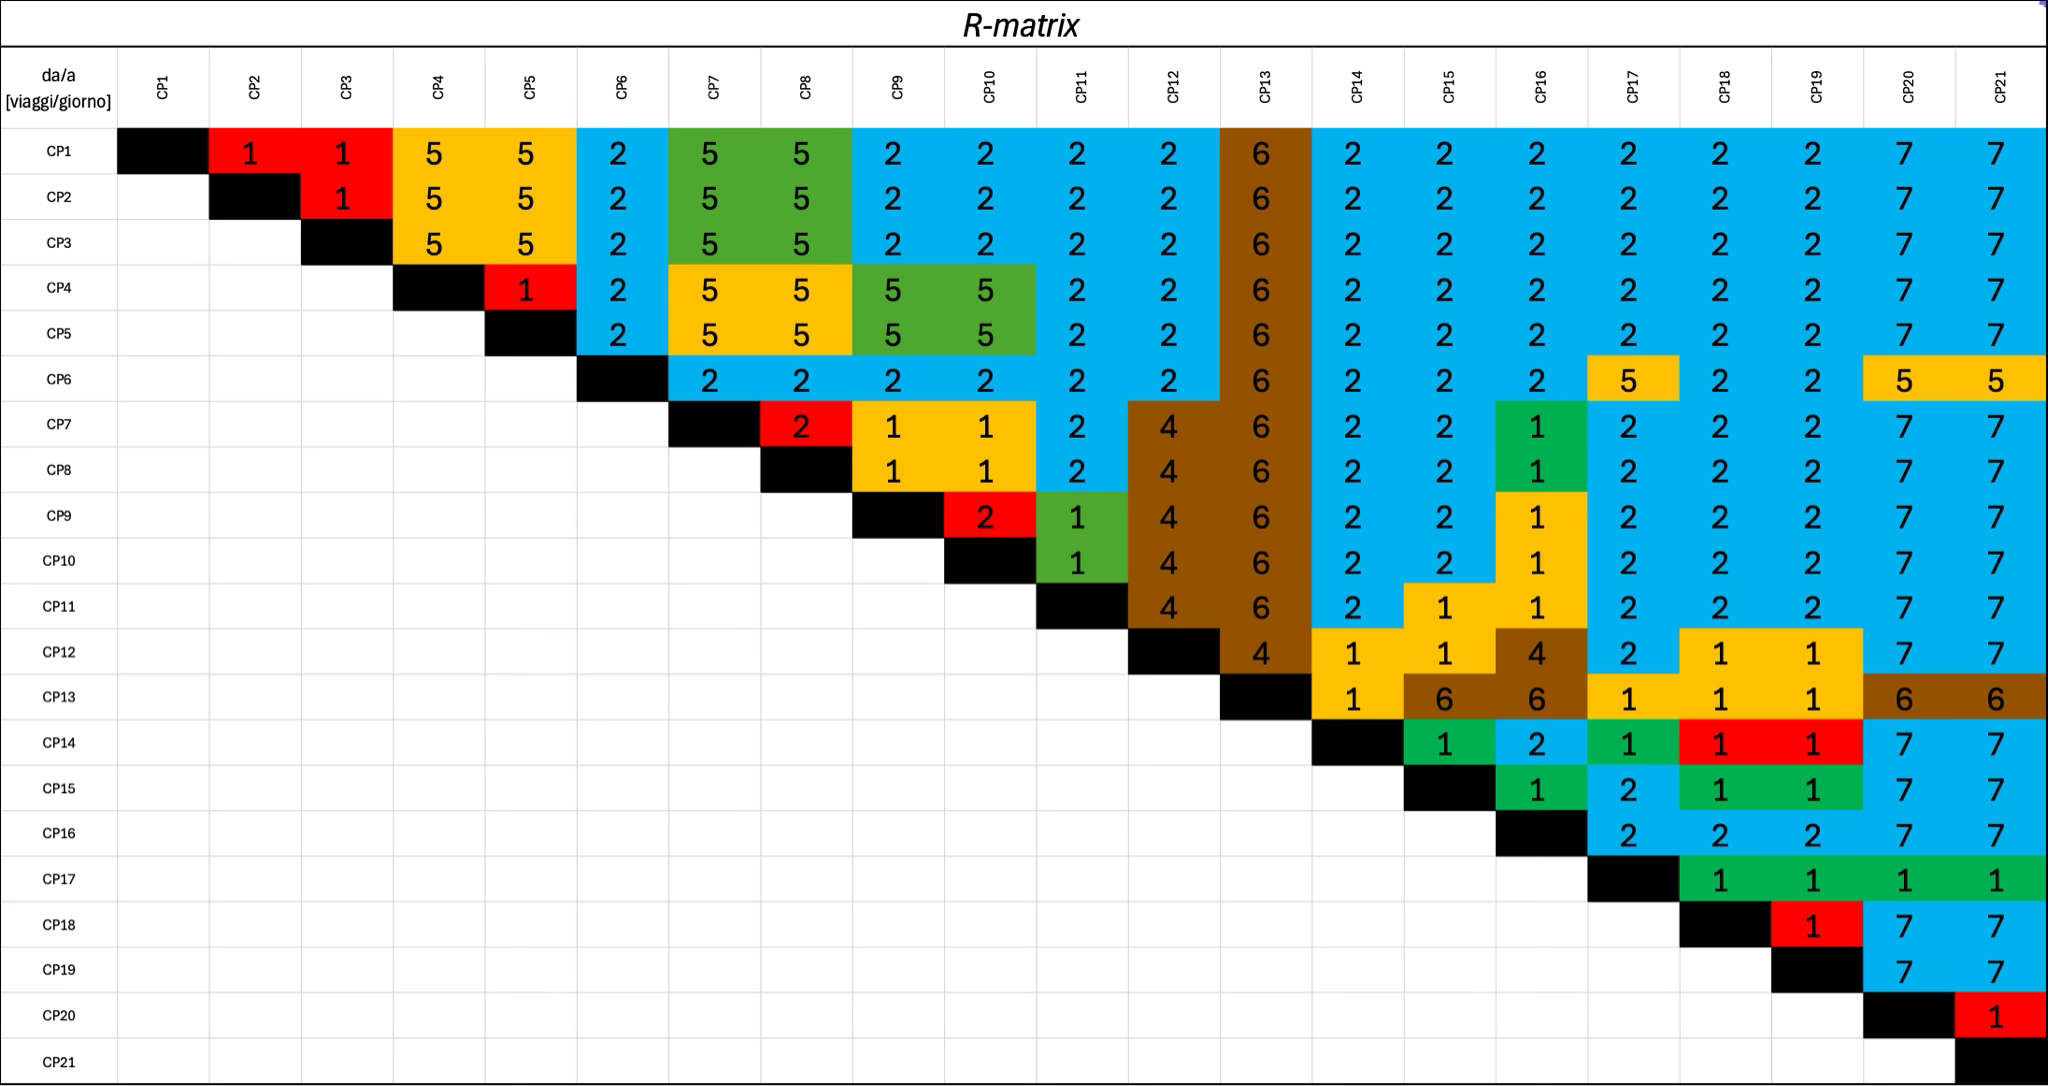
\includegraphics[width=0.7\textwidth]{R-Matrix Numbers.png}
  \caption{R-Matrix}
  \label{fig:R-Matrix Numbers}
\end{figure}
\begin{figure}[H]
  \centering
  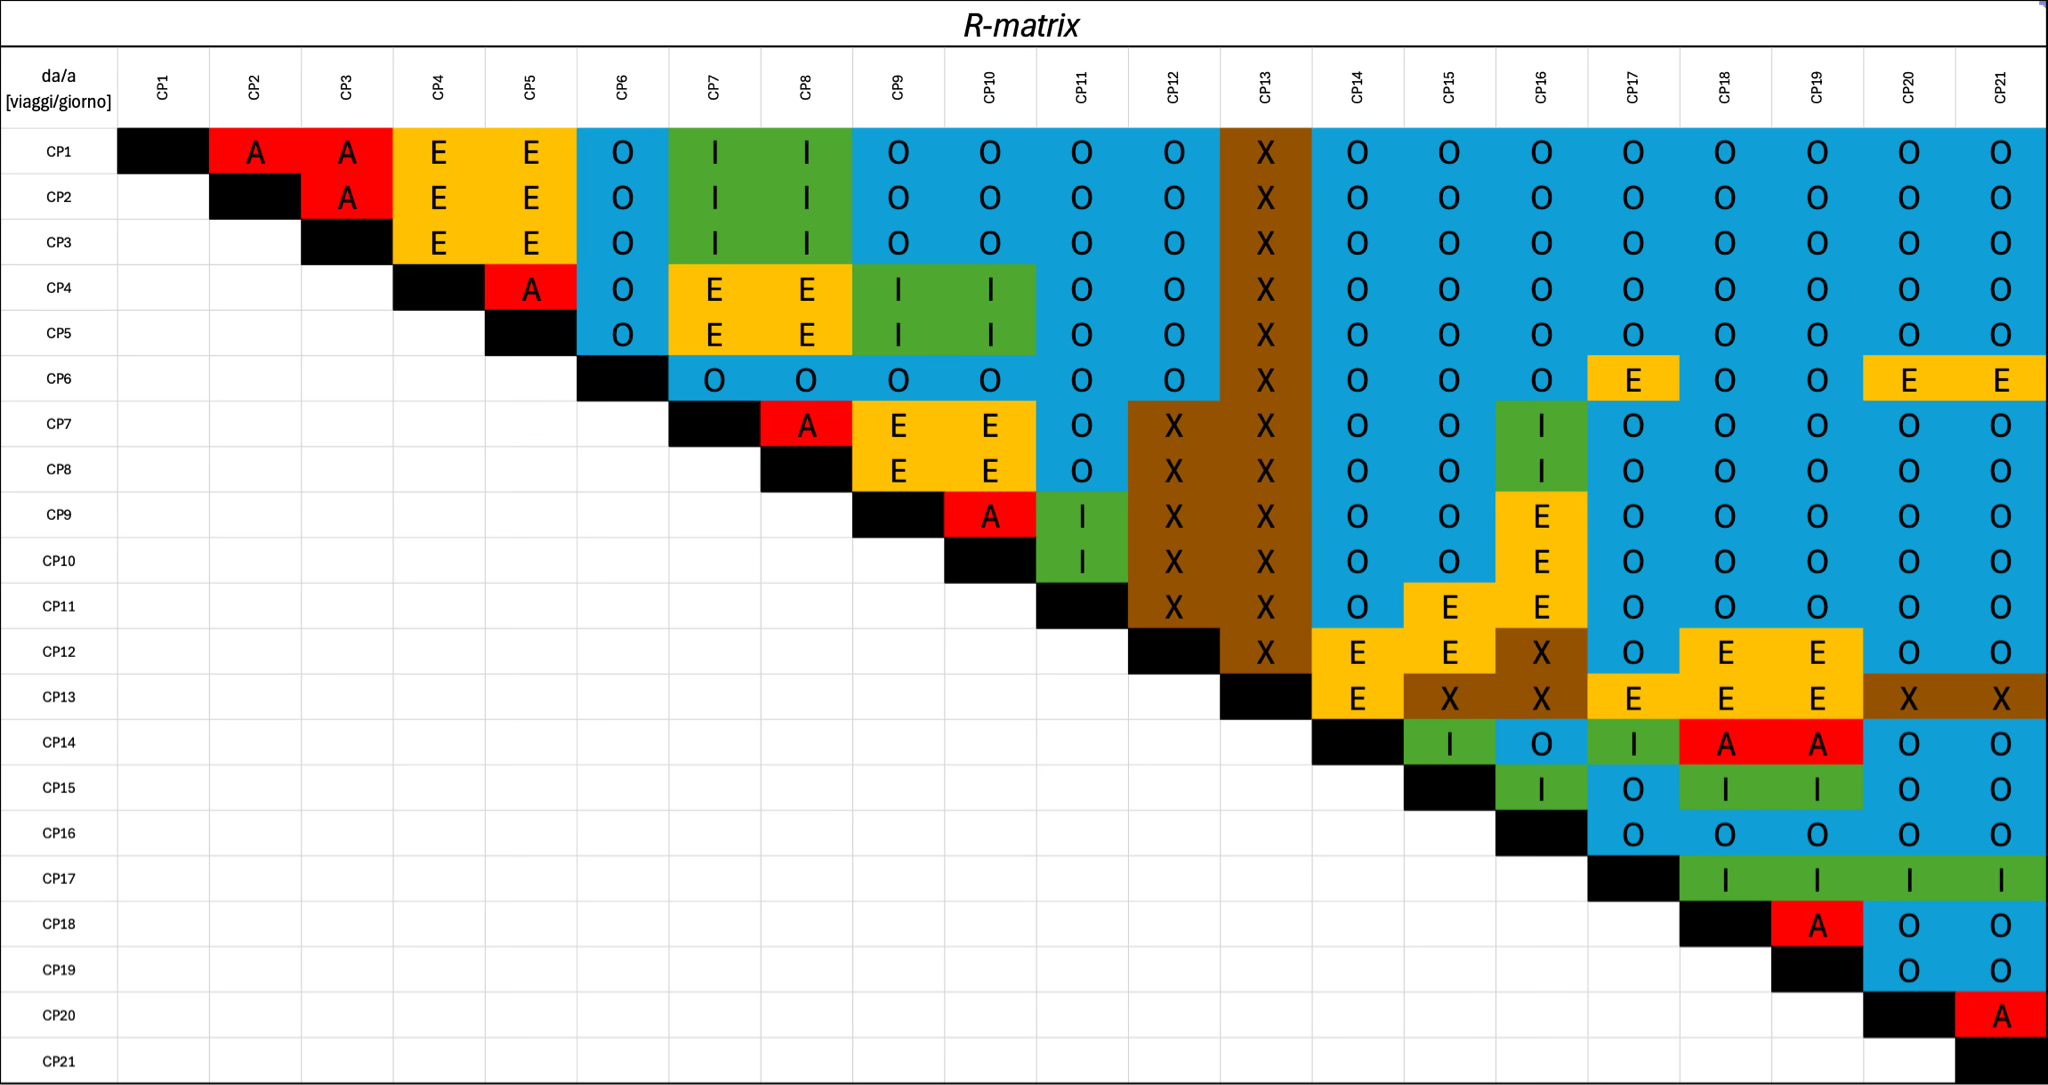
\includegraphics[width=0.7\textwidth]{R-Matrix Values.png}
  \caption{R-Matrix valori}
  \label{fig:R-Matrix Values}
\end{figure}
\subsubsection*{Triangoli di Buff}
Questi sono i due triangoli di Buff che rappresentano le due matrici, la P-Matrix e la R-Matrix.
\begin{figure}[H]
  \centering
  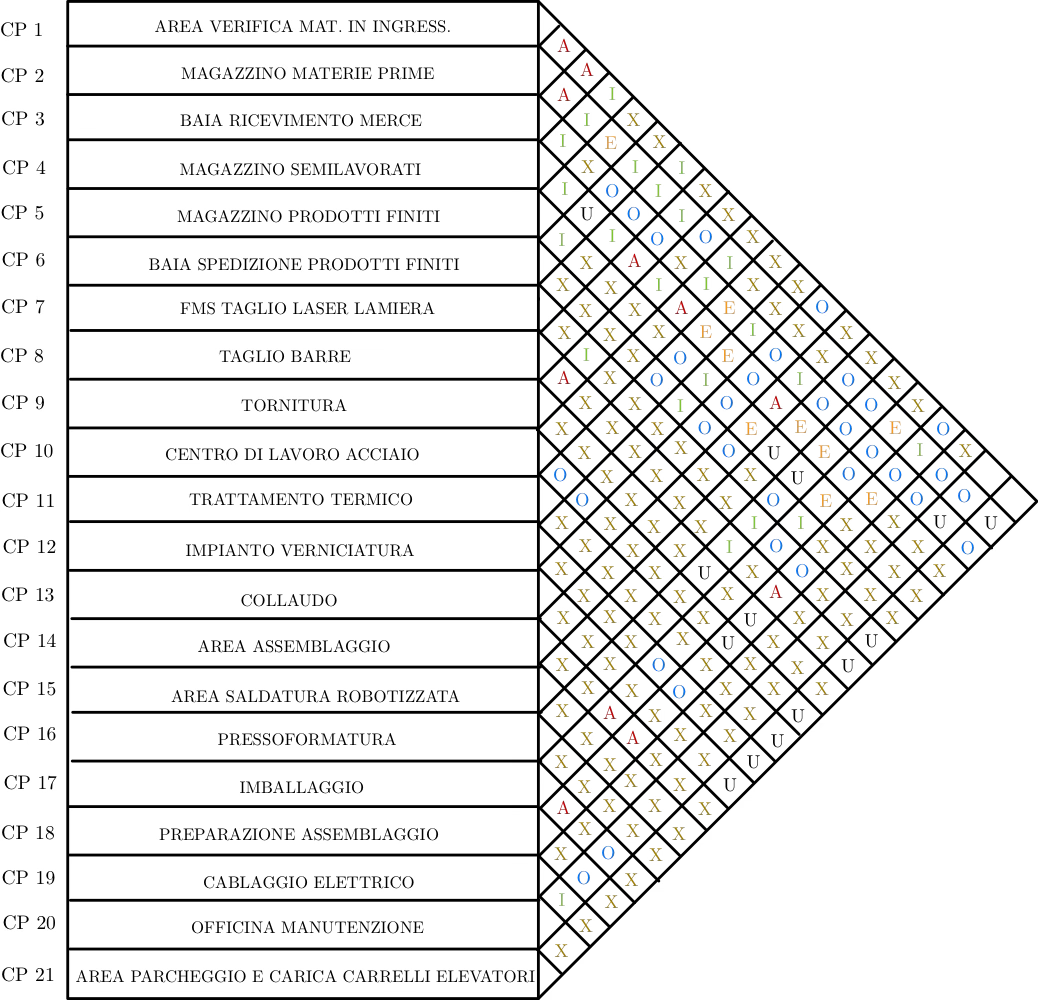
\includegraphics[width=0.7\textwidth]{P-Matrix Buff.png}
  \caption{P-Matrix Buff}
  \label{fig:P-Matrix Buff}
\end{figure}
\begin{figure}[H]
  \centering
  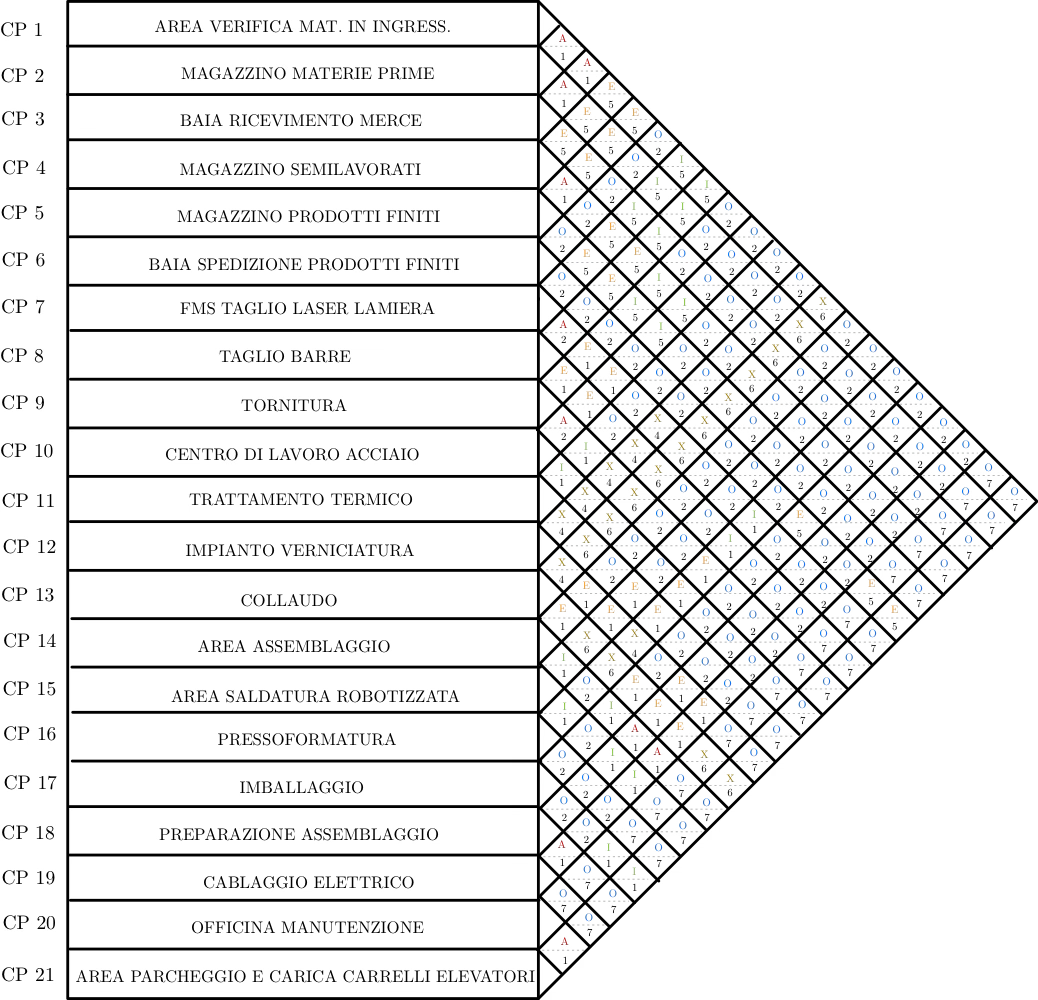
\includegraphics[width=0.7\textwidth]{R-Matrix Buff.png}
  \caption{R-Matrix Buff}
  \label{fig:R-Matrix Buff}
\end{figure}
La somma delle due matrici fornisce la S-Matrix che permette di calcolare il ranking dei CP.
\begin{figure}[H]
  \centering
  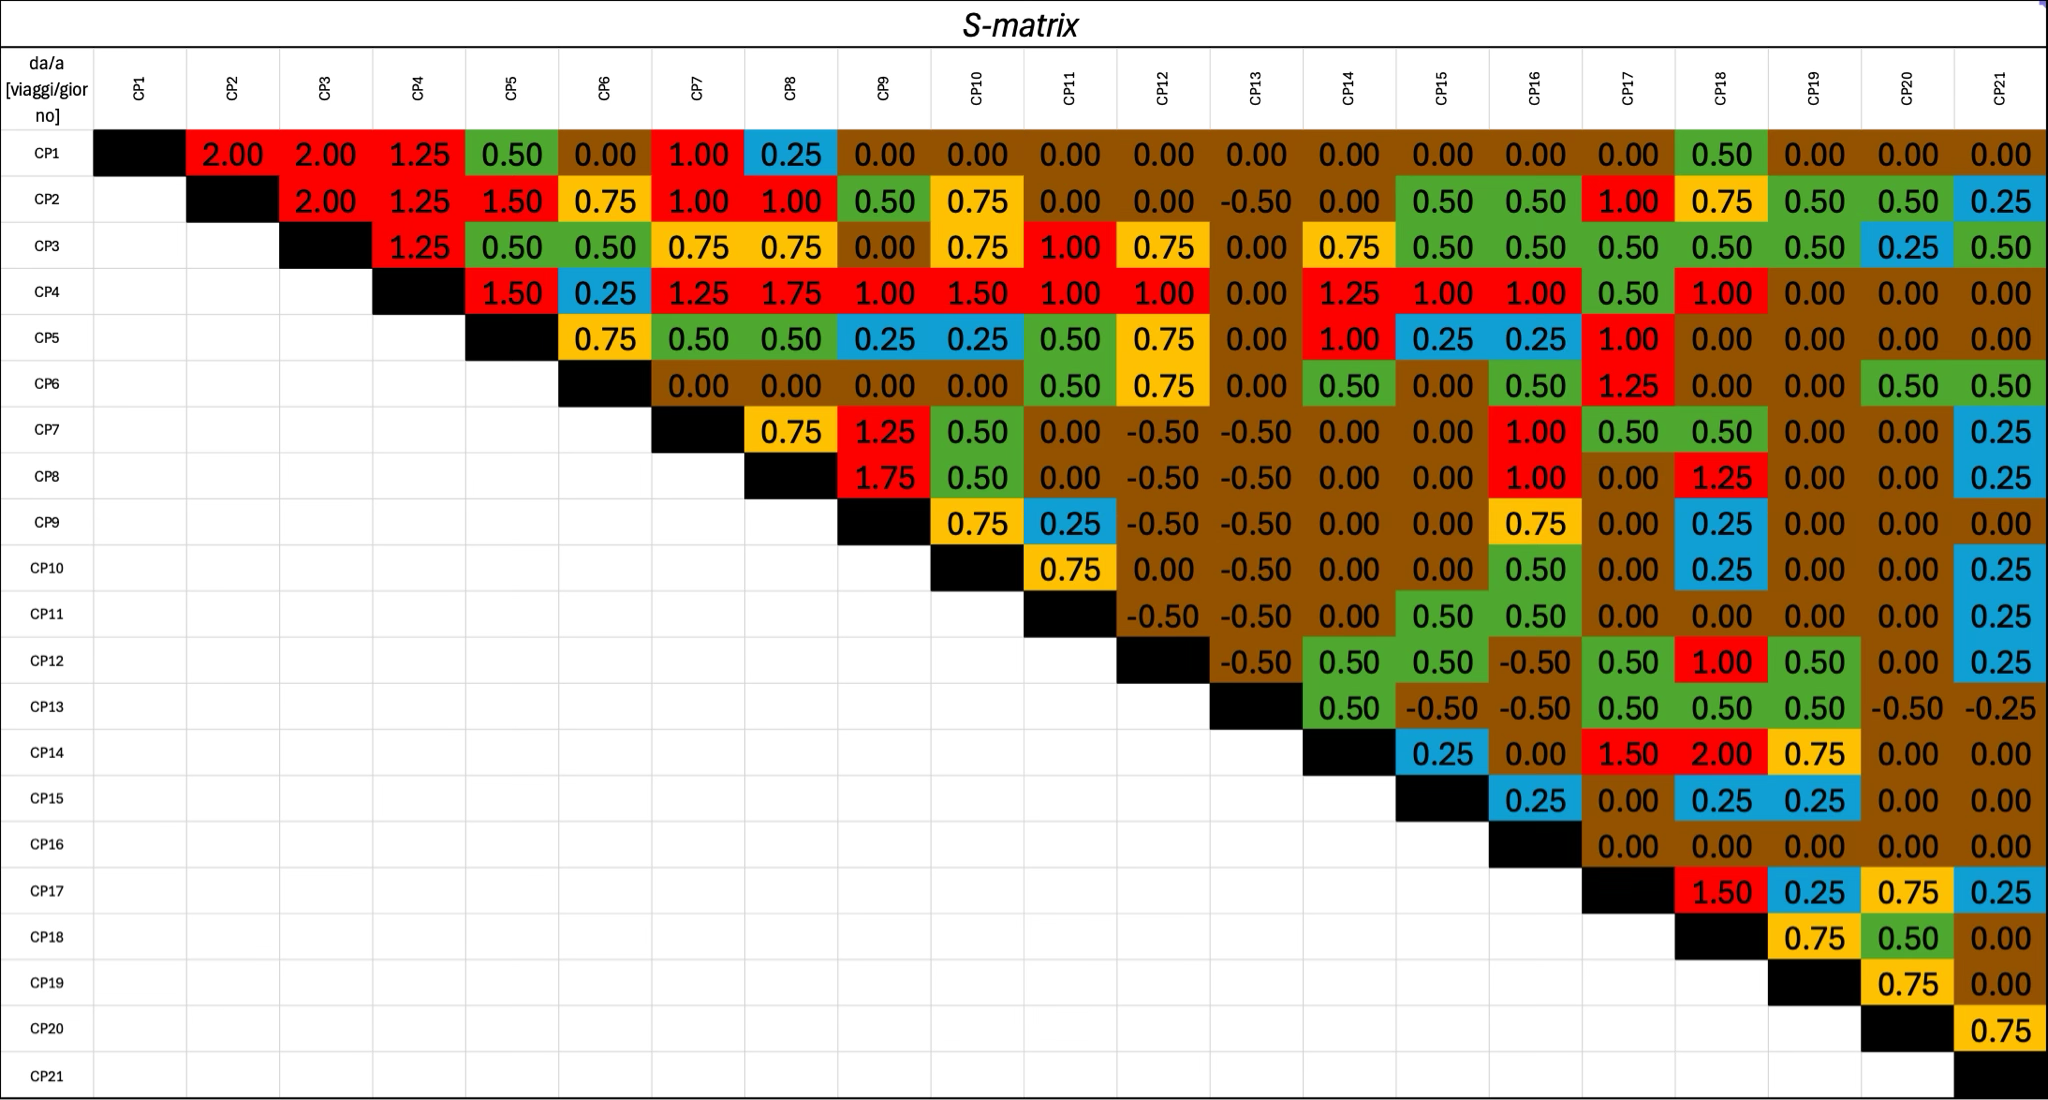
\includegraphics[width=0.6\textwidth]{S-Matrix.png}
  \caption{S-Matrix }
  \label{fig:S-Matrix}
\end{figure}
\subsubsection*{Ranking dei Control Point}
Dalla S-Matrix si ottiene il ranking dei control point, che permette di ordinare i CP in base alla loro importanza, considerando sia i flussi di materiali che le relazioni interfunzionali.
\begin{figure}[H]
  \centering
  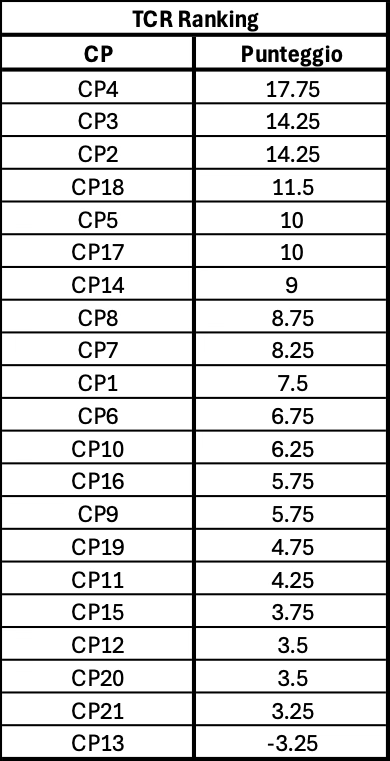
\includegraphics[width=0.4\textwidth]{TCR Ranking.png}
  \caption{Ranking dei Control Point}
  \label{fig:Ranking dei Control Point}
\end{figure}
\subsubsection*{Ordine di posizionamento dei Control Point}
Dall'analisi del ranking dei control point, si ottiene l'ordine di inserimento dei CP, che indica la sequenza in cui i CP devono essere posizionati nel layout.
\begin{figure}[H]
  \centering
  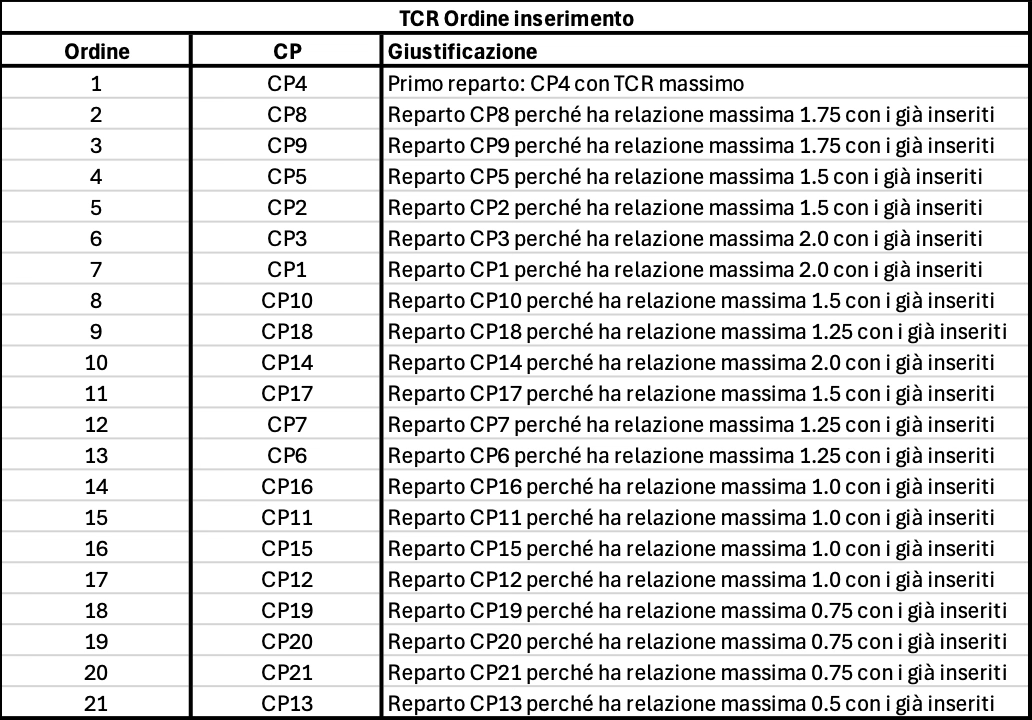
\includegraphics[width=0.7\textwidth]{TCR Inserimento.png}
  \caption{Ordine di posizionamento dei Control Point}
  \label{fig:Ordine di posizionamento dei Control Point}
\end{figure}
\subsection{Step 2: Positioning}
Dopo aver ottenuto l'ordine di posizionamento dei CP, si procede con il posizionamento dei CP nel layout, in base all'algoritmo TCR, ottenendo il diagramma di rapporti tra le attività.
\begin{figure}[H]
  \centering
  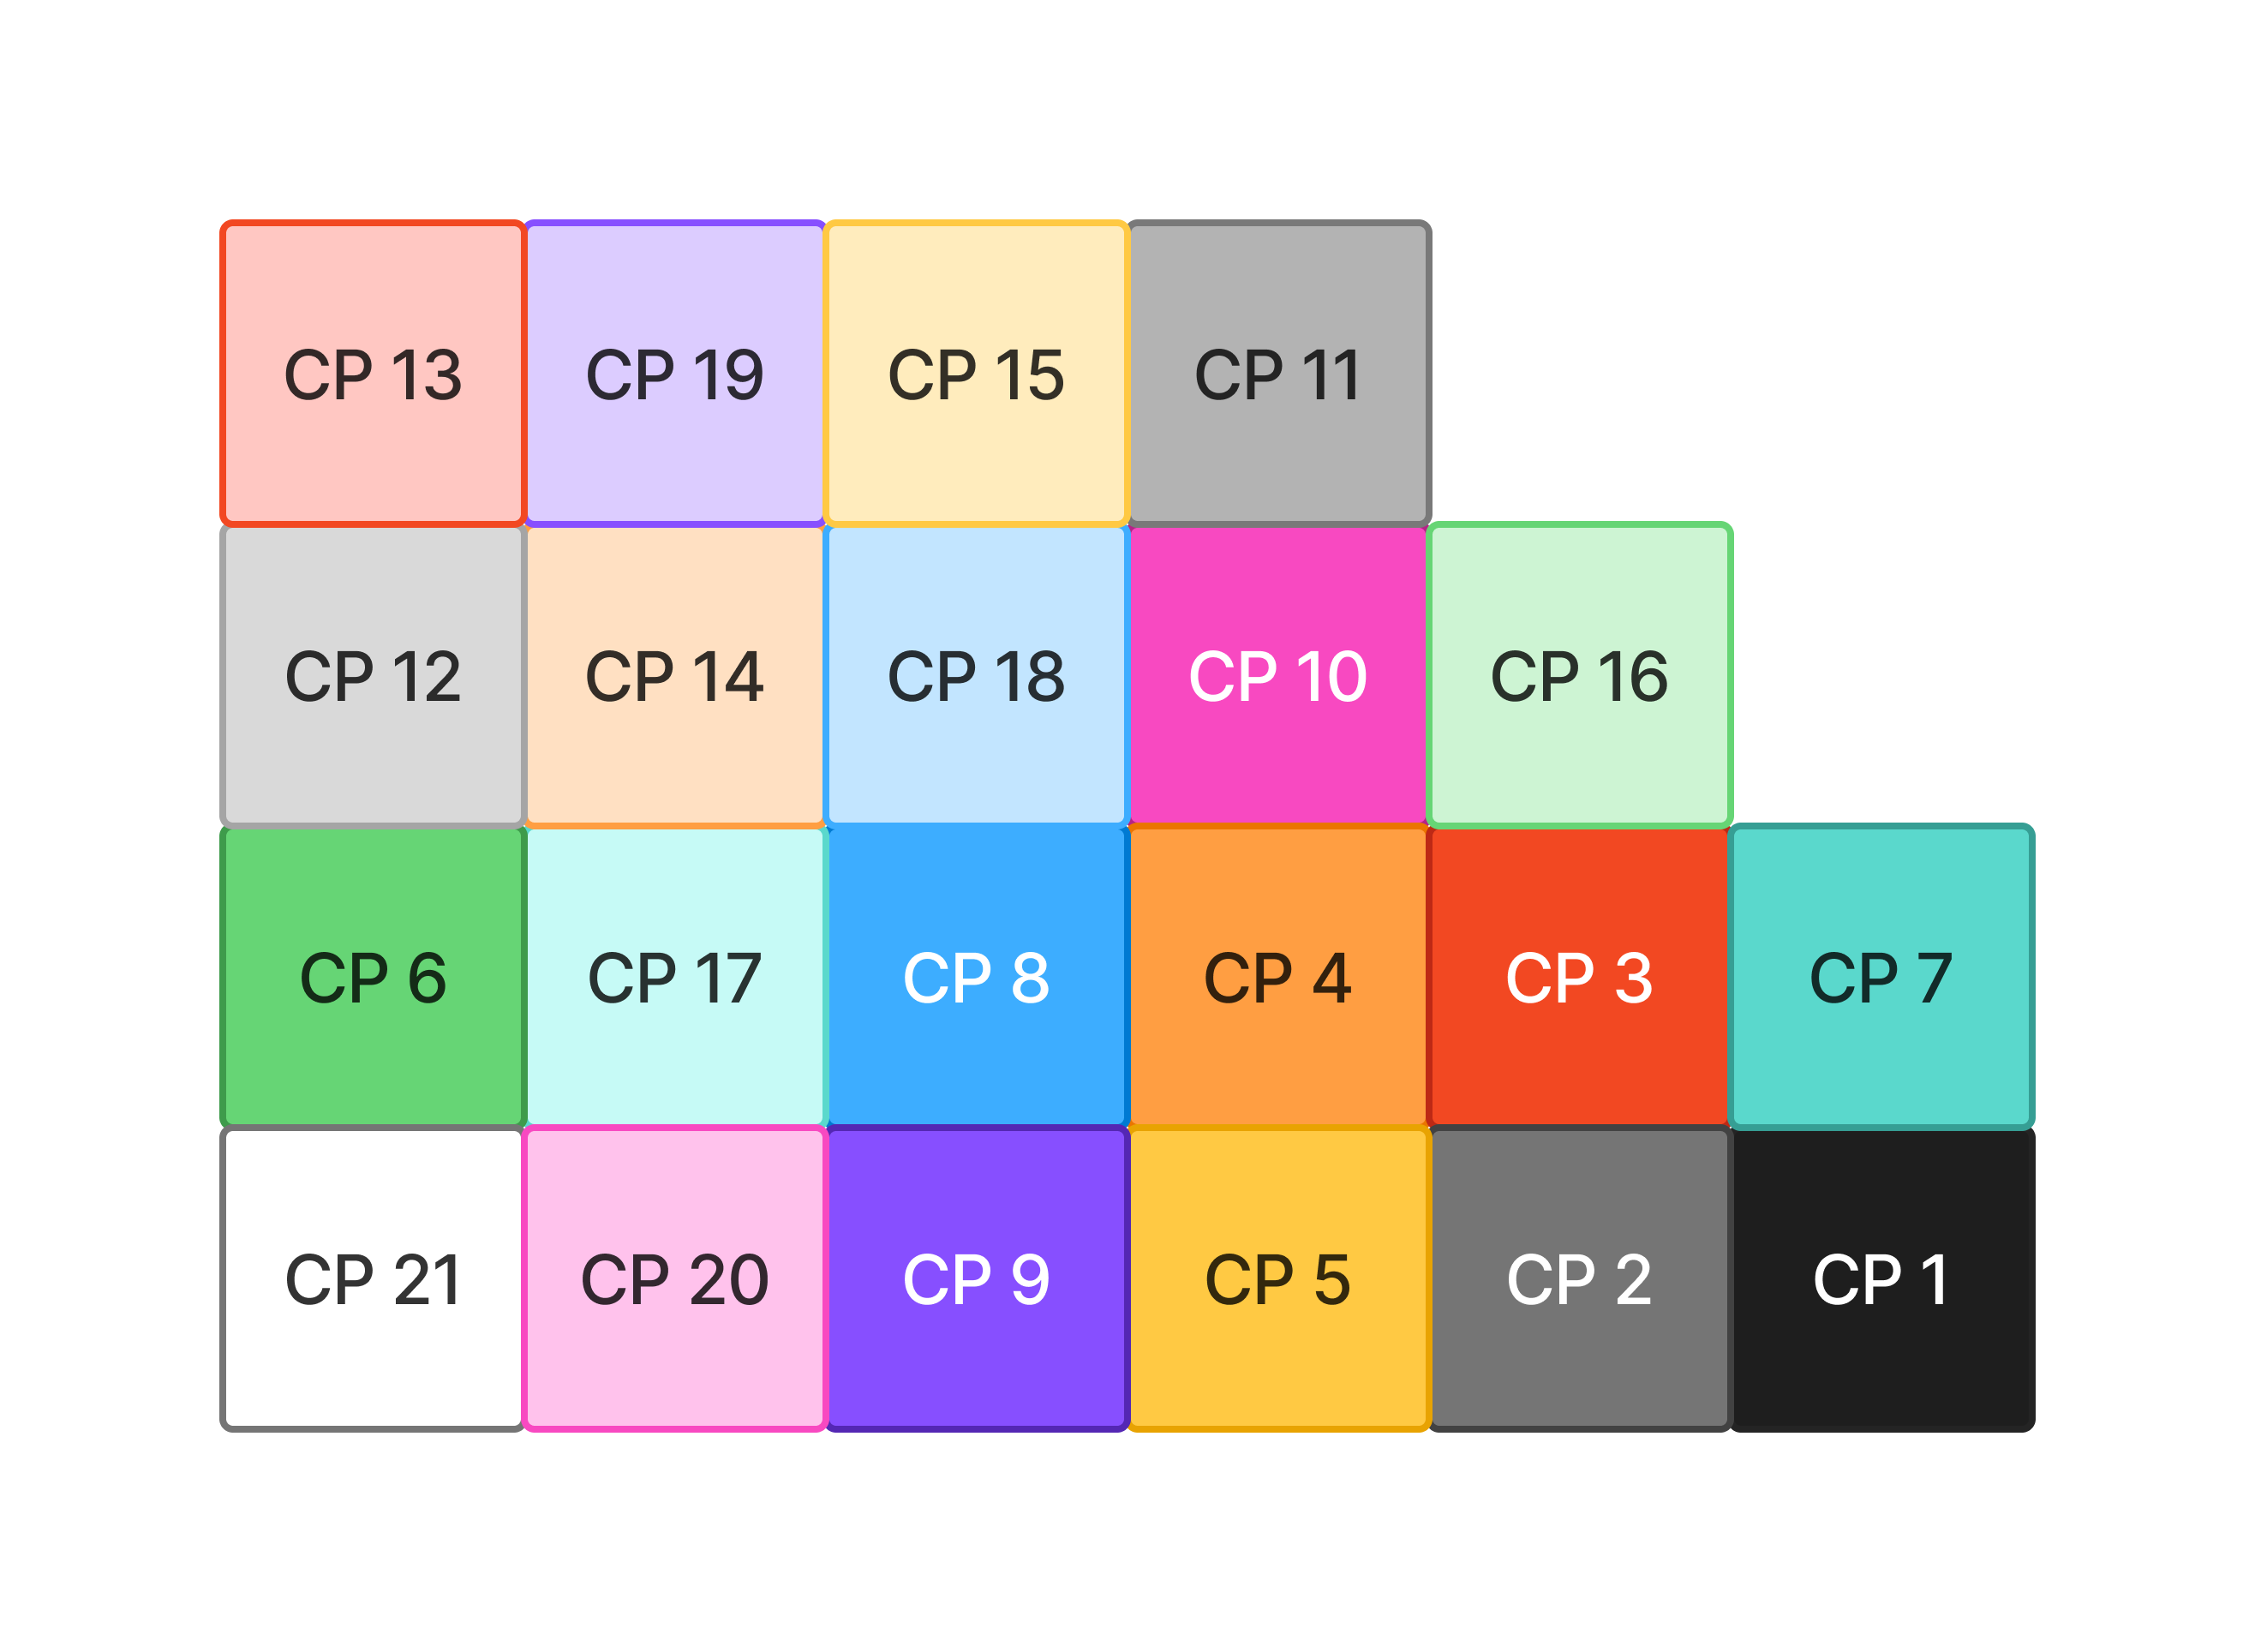
\includegraphics[width=0.7\textwidth]{TCR Positioning.png}
  \caption{Diagramma di rapporti tra le attività}
  \label{fig:Diagramma di rapporti tra le attività}
\end{figure}
\subsection{Step 3: Layout}
Infine, si procede con la costruzione secondo una logica funzionale alla sequenza delle attività svolte del layout vero e proprio.
\begin{figure}[H]
  \centering
  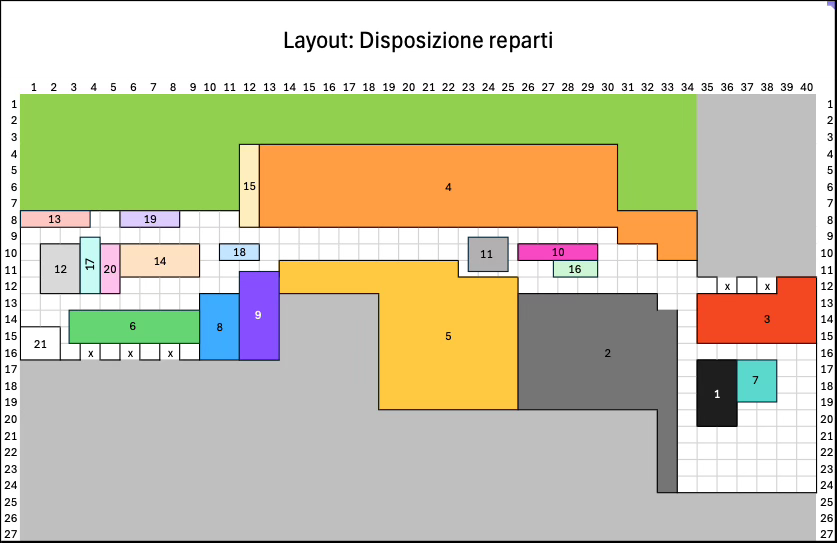
\includegraphics[width=1\textwidth]{Layout disposizione.png}
  \caption{Layout finale}
  \label{fig:Layout finale}
\end{figure}
\section{Quantificazione del costo di movimentazione globale}
Abbiamo calcolato il costo di movimentazione globale, espresso in metri/giorno, con riferimento alla soluzione di layout proposta e rispettivamente nei seguenti due distinti casi:
\begin{enumerate}
  \item CASO A: rispettando l’ubicazione scelta per i control point;
  \item CASO B: pensando l’I/O di tutti i reparti concentrati nel relativo baricentro. Tale ipotesi adottarla in ogni caso ove esplicitamente indicato in Tabella 1.
\end{enumerate}
\subsection{CASO A: Ubicazione scelta per i control point}
Per calcolare il costo di movimentazione globale nel caso A, abbiamo considerato l'ubicazione scelta per i control point, utilizzando i flussi di materiali e le distanze tra i reparti in modo che fosse comodo lo scambio tra i flussi, eccetto per i reparti in cui era specificato un control point di tipo baricentrico.
Si ottiene il seguente layout:
\begin{figure}[H]
  \centering
  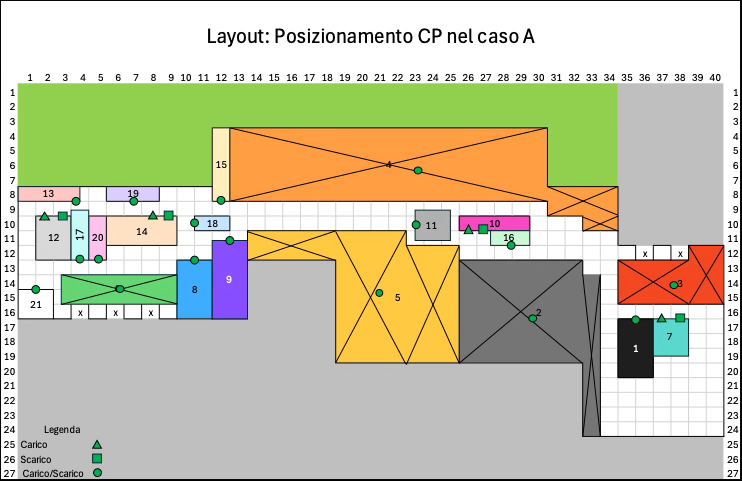
\includegraphics[width=1\textwidth]{Layout caso A.png}
  \caption{Layout A: Ubicazione scelta per i control point}
  \label{fig:Layout A}
\end{figure}
Abbiamo poi estratto le coordinate dei control point, che sono state utilizzate per calcolare le distanze tra i reparti e i flussi di materiali, ottenendo il seguente risultato:
\begin{figure}[H]
  \centering
  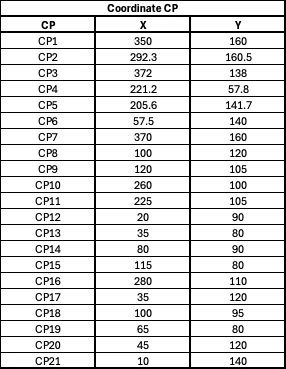
\includegraphics[width=0.3\textwidth]{Coordinate CP 1.png}
  \caption{Coordinate dei Control Point}
  \label{fig:Coordinate dei Control Point}
\end{figure}
Le distanze rettangolari tra i control point sono calcolate tramite la seguente formula:

\begin{equation*}
  d_{ij} = |x_i - x_j| + |y_i - y_j|
\end{equation*}

dove $d_{ij}$ è la distanza rettangolare tra il control point $i$ e il control point $j$, mentre $(x_i, y_i)$ e $(x_j, y_j)$ sono le coordinate dei rispettivi control point.
Queste distanze vengono poi utilizzate per calcolare il costo di movimentazione globale, moltiplicando ciascun flusso $f_{ij}$ per la distanza $d_{ij}$ tra i reparti:
\begin{equation*}
  D_{TOT_{A}} = \sum_{i,j} f_{ij} \cdot d_{ij}
\end{equation*}
Dove $D_{TOT_{A}}$ viene ottenuto moltiplicando le due matrici, la matrice dei flussi e la matrice delle distanze, ottenendo le due matrici:
\begin{figure}[H]
  \centering
  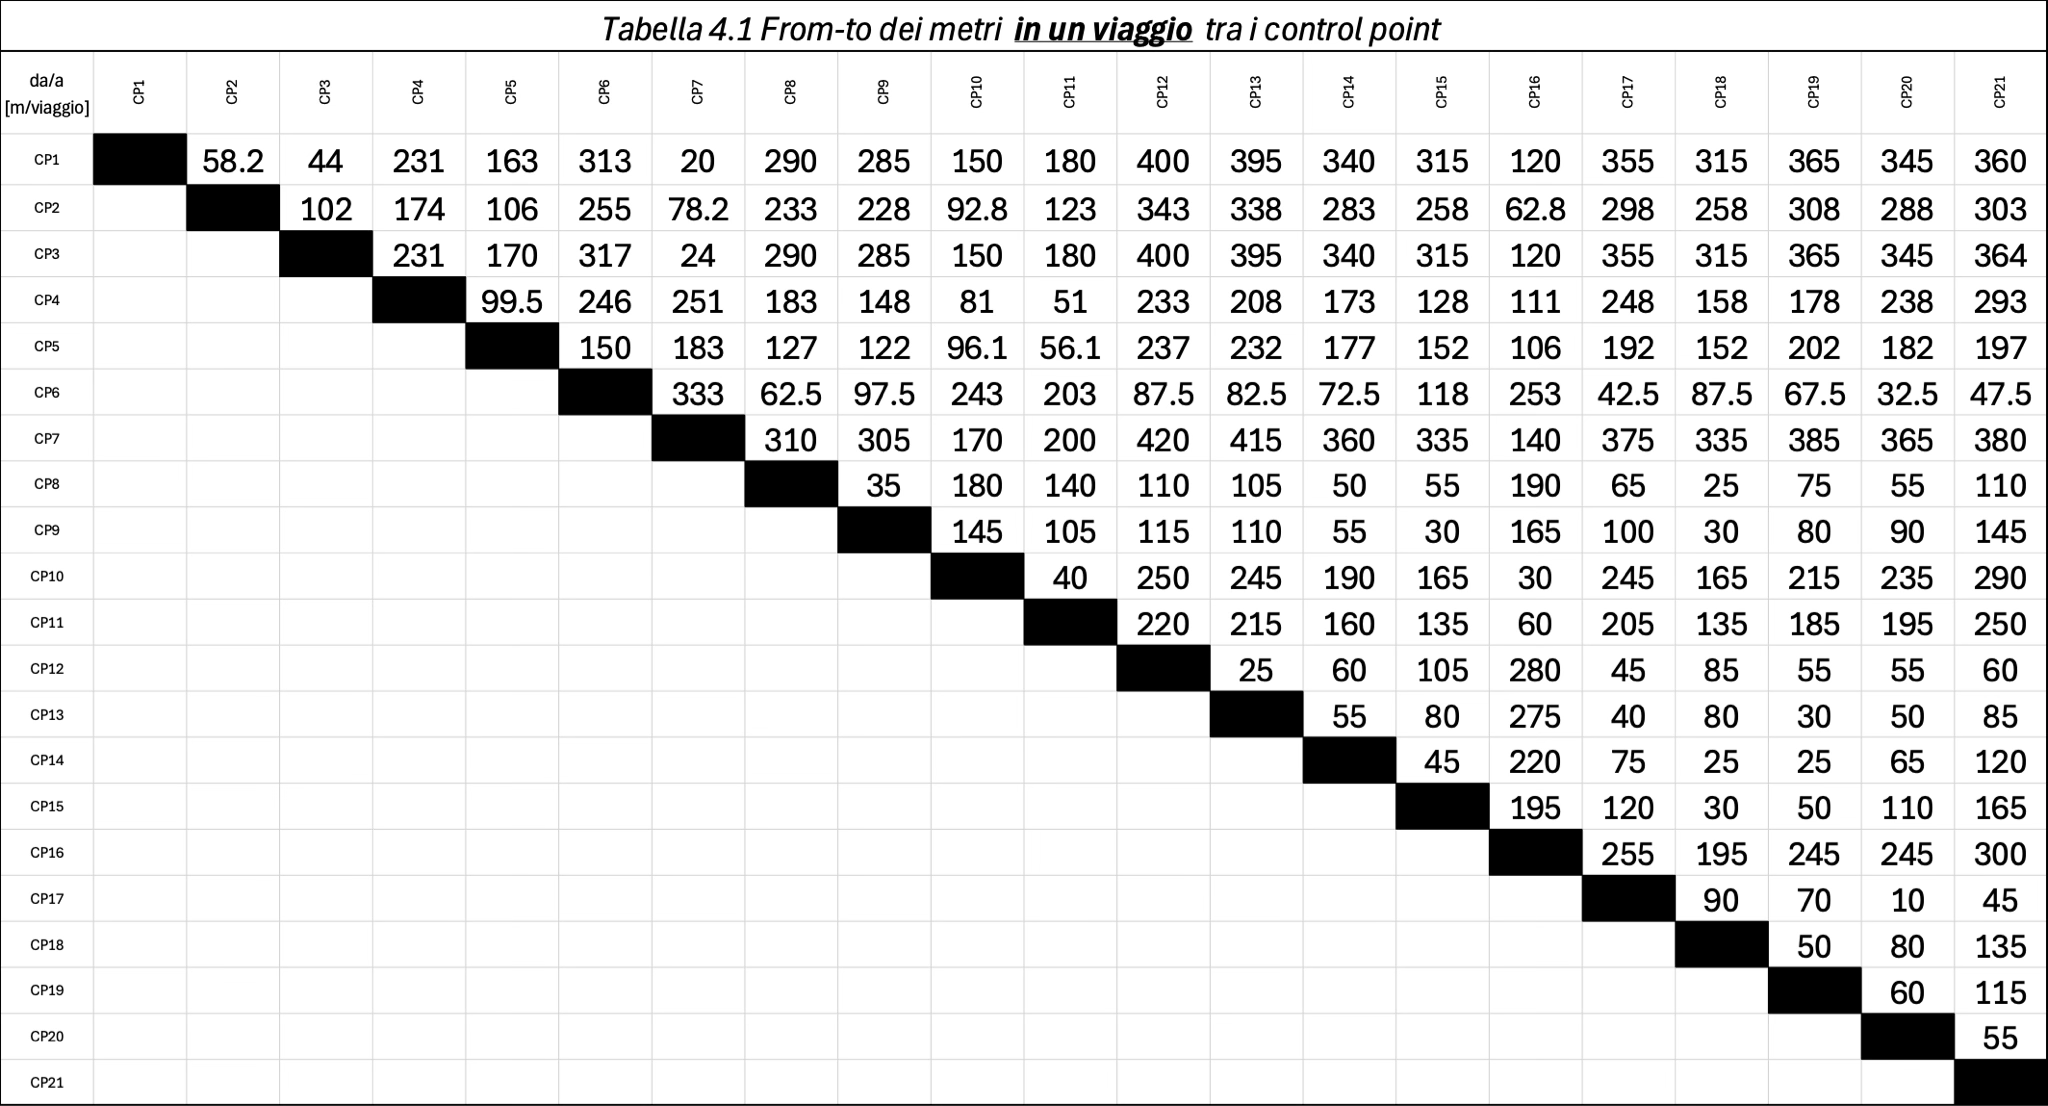
\includegraphics[width=0.7\textwidth]{Tabella 4.1.1.png}
  \caption{From-To dei metri in un viaggio tra control point}
  \label{fig:From-To dei metri in un viaggio tra control point}
\end{figure}
\begin{figure}[H]
  \centering
  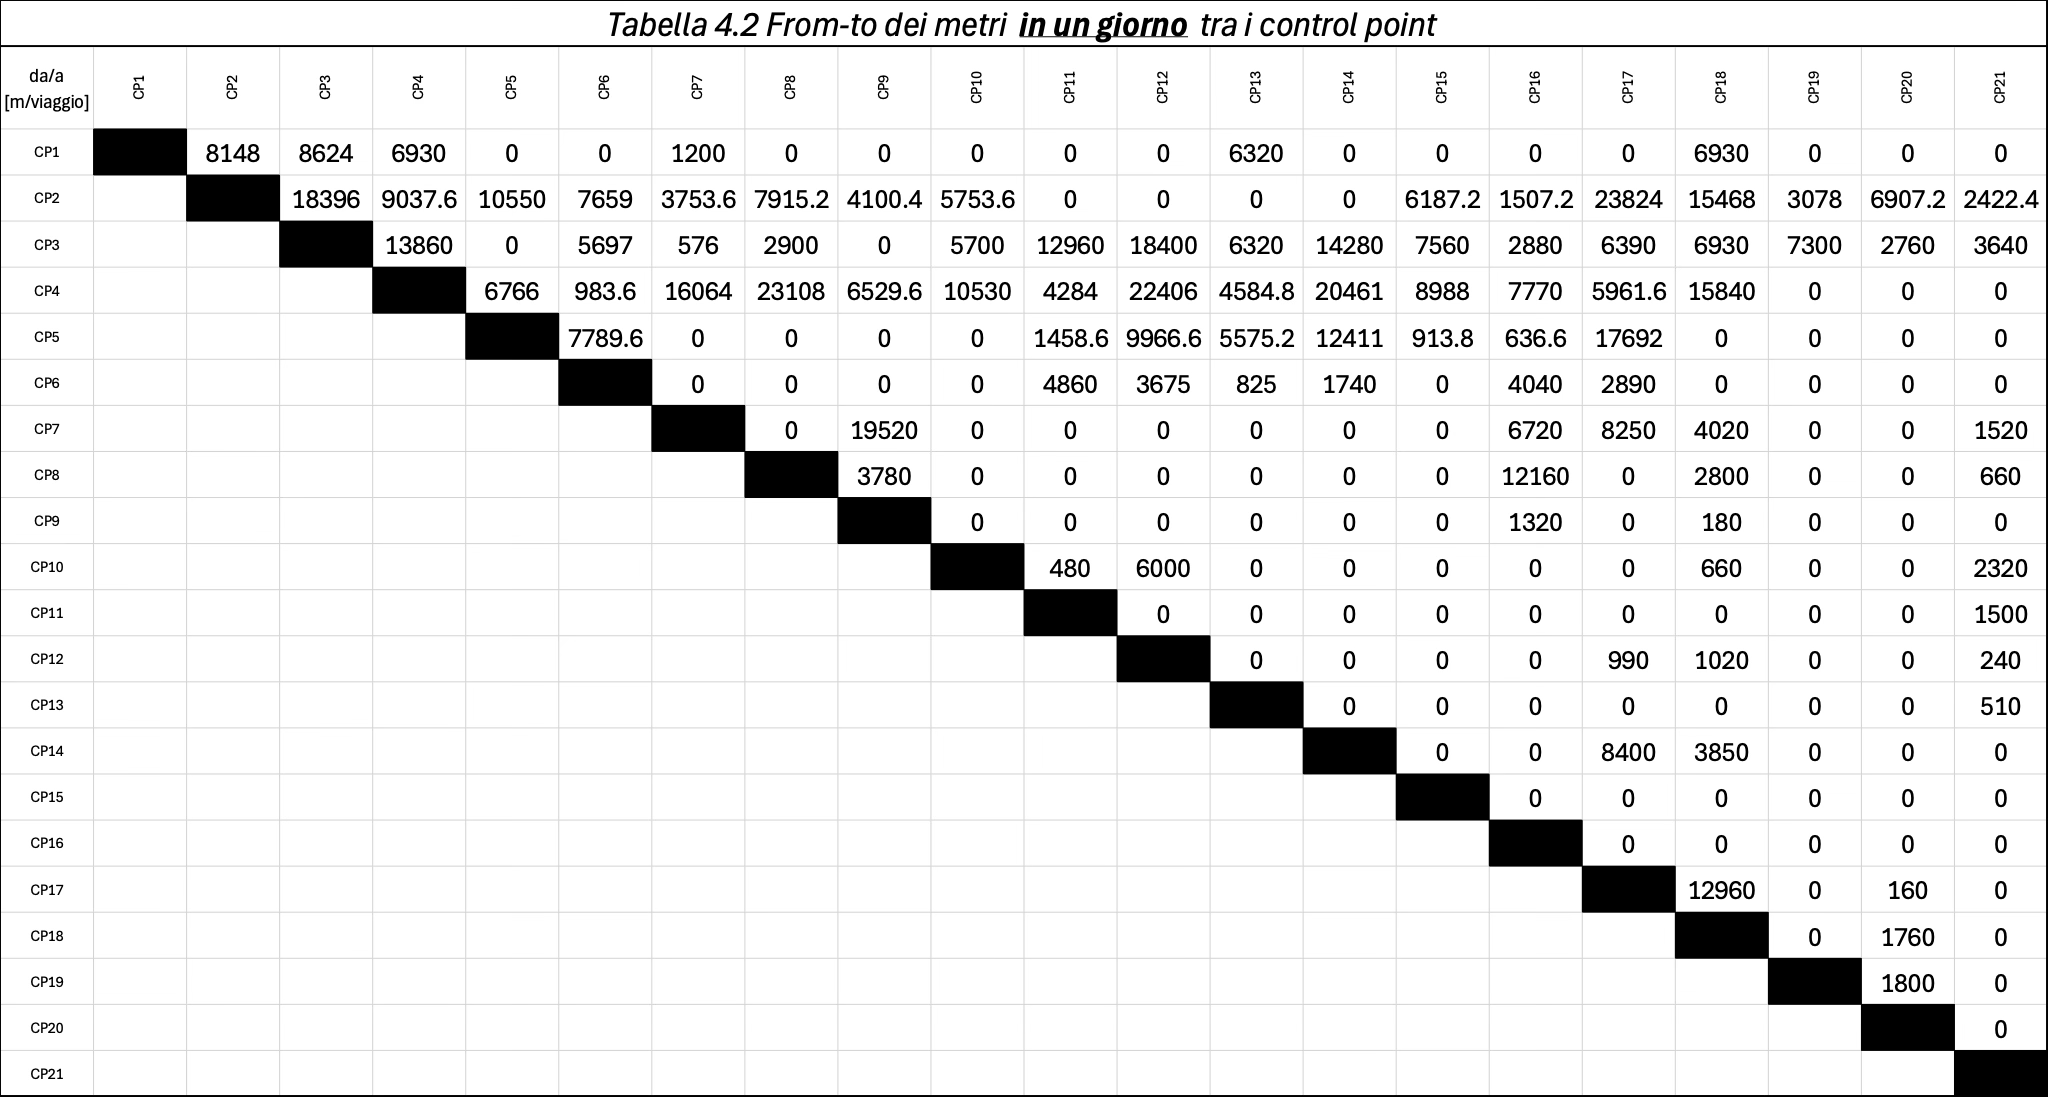
\includegraphics[width=0.7\textwidth]{Tabella 4.1.2.png}
  \caption{From-To dei metri in un giorno tra control point}
  \label{fig:From-To dei metri in un giorno tra control point 2}
\end{figure}
Il costo di movimentazione globale nel caso A è quindi:
\begin{equation*}
  D_{TOT_{A}} = 615195 \left[\frac{\mathrm{m}}{\mathrm{giorno}}\right]
\end{equation*}
\subsection{CASO B: I/O di tutti i reparti concentrati nel relativo baricentro}
Per calcolare il costo di movimentazione globale nel caso B, abbiamo considerato l'ubicazione dei control point come il baricentro dei reparti, in modo da concentrare l'I/O di tutti i reparti in un unico punto.
Si ottiene il seguente layout:
\begin{figure}[H]
  \centering
  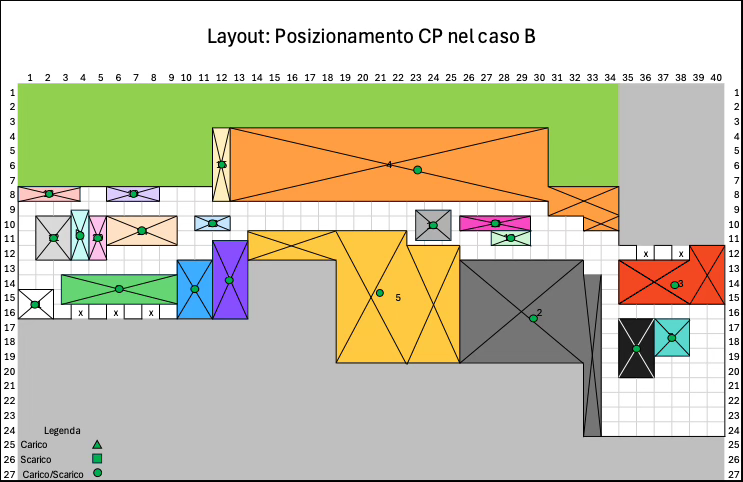
\includegraphics[width=1\textwidth]{Layout caso B.png}
  \caption{Layout B: I/O di tutti i reparti concentrati nel relativo baricentro}
  \label{fig:Layout B}
\end{figure}
Le coordinate dei control point sono state calcolate come il baricentro dei reparti, ottenendo le seguenti coordinate:
\begin{figure}[H]
  \centering
  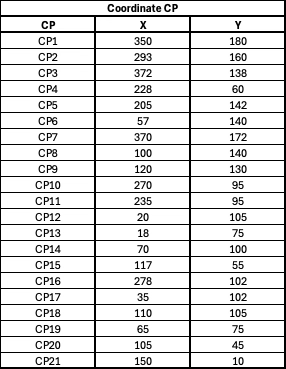
\includegraphics[width=0.3\textwidth]{Coordinate CP 2.png}
  \caption{Coordinate dei Control Point nel caso B}
  \label{fig:Coordinate dei Control Point B}
\end{figure}
Le distanze rettangolari tra i control point sono calcolate tramite la stessa formula utilizzata nel caso A:
\begin{equation*}
  d_{ij} = |x_i - x_j| + |y_i - y_j|
\end{equation*}
Queste distanze vengono poi utilizzate per calcolare il costo di movimentazione globale, moltiplicando ciascun flusso $f_{ij}$ per la distanza $d_{ij}$ tra i reparti:
\begin{equation*}
  D_{TOT_{B}} = \sum_{i,j} f_{ij} \cdot d_{ij}
\end{equation*}
Dove $D_{TOT_{B}}$ viene ottenuto moltiplicando le due matrici, la matrice dei flussi e la matrice delle distanze, ottenendo le due matrici:
\begin{figure}[H]
  \centering
  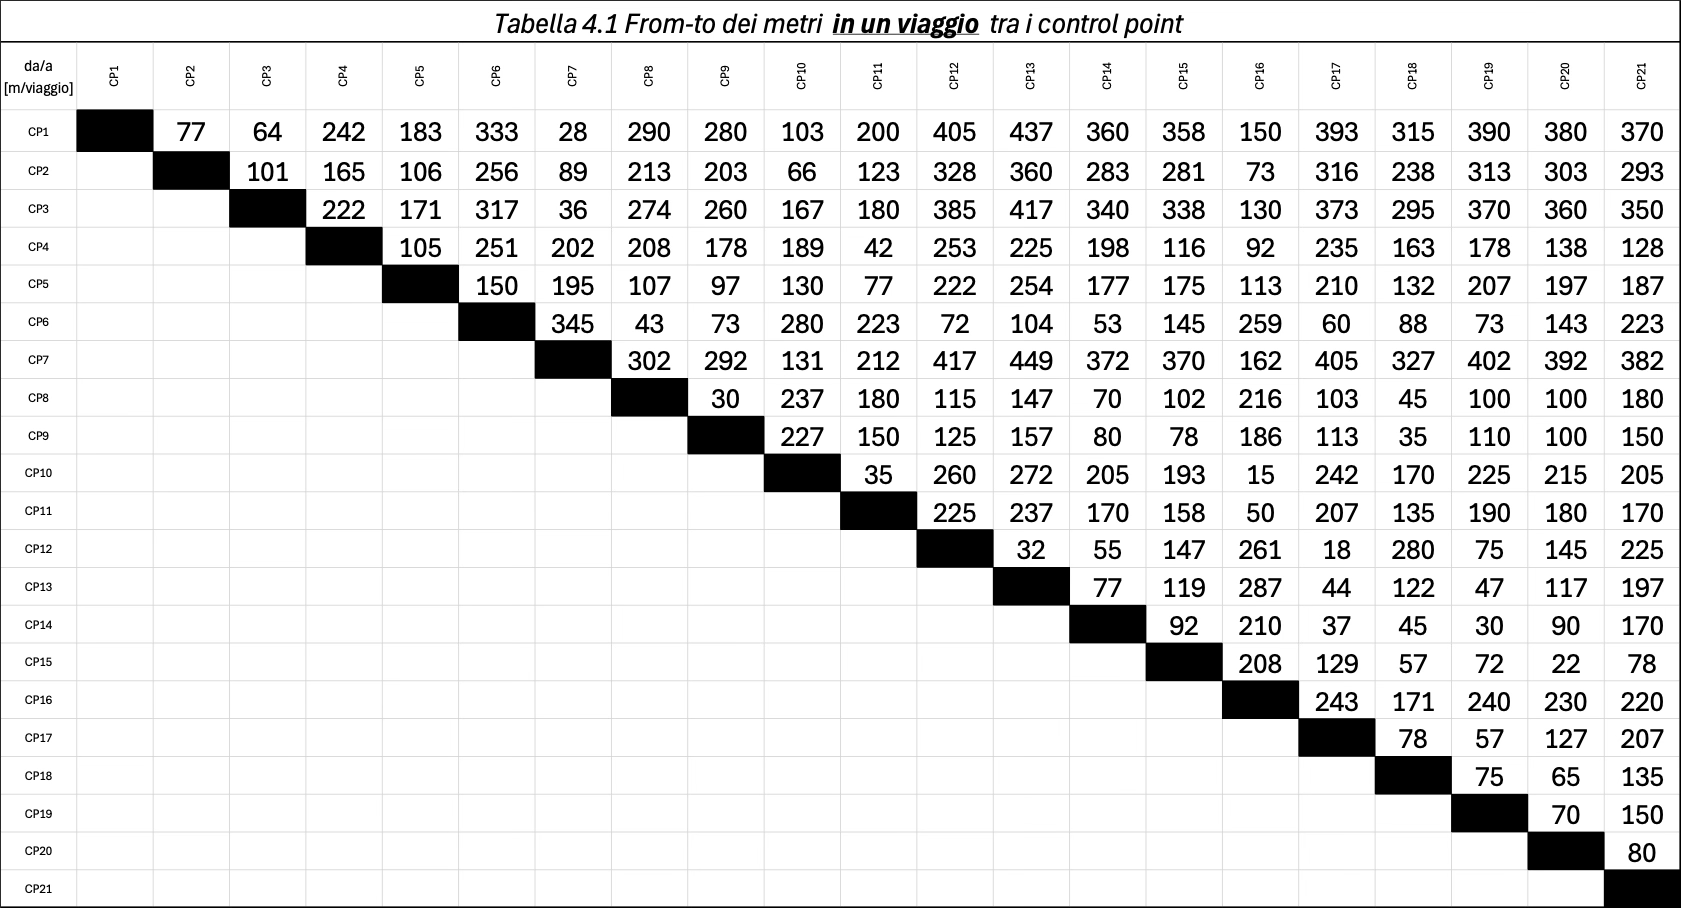
\includegraphics[width=0.7\textwidth]{Tabella 4.2.1.png}
  \caption{From-To dei metri in un viaggio tra control point nel caso B}
  \label{fig:From-To dei metri in un viaggio tra control point B}
\end{figure}
\begin{figure}[H]
  \centering
  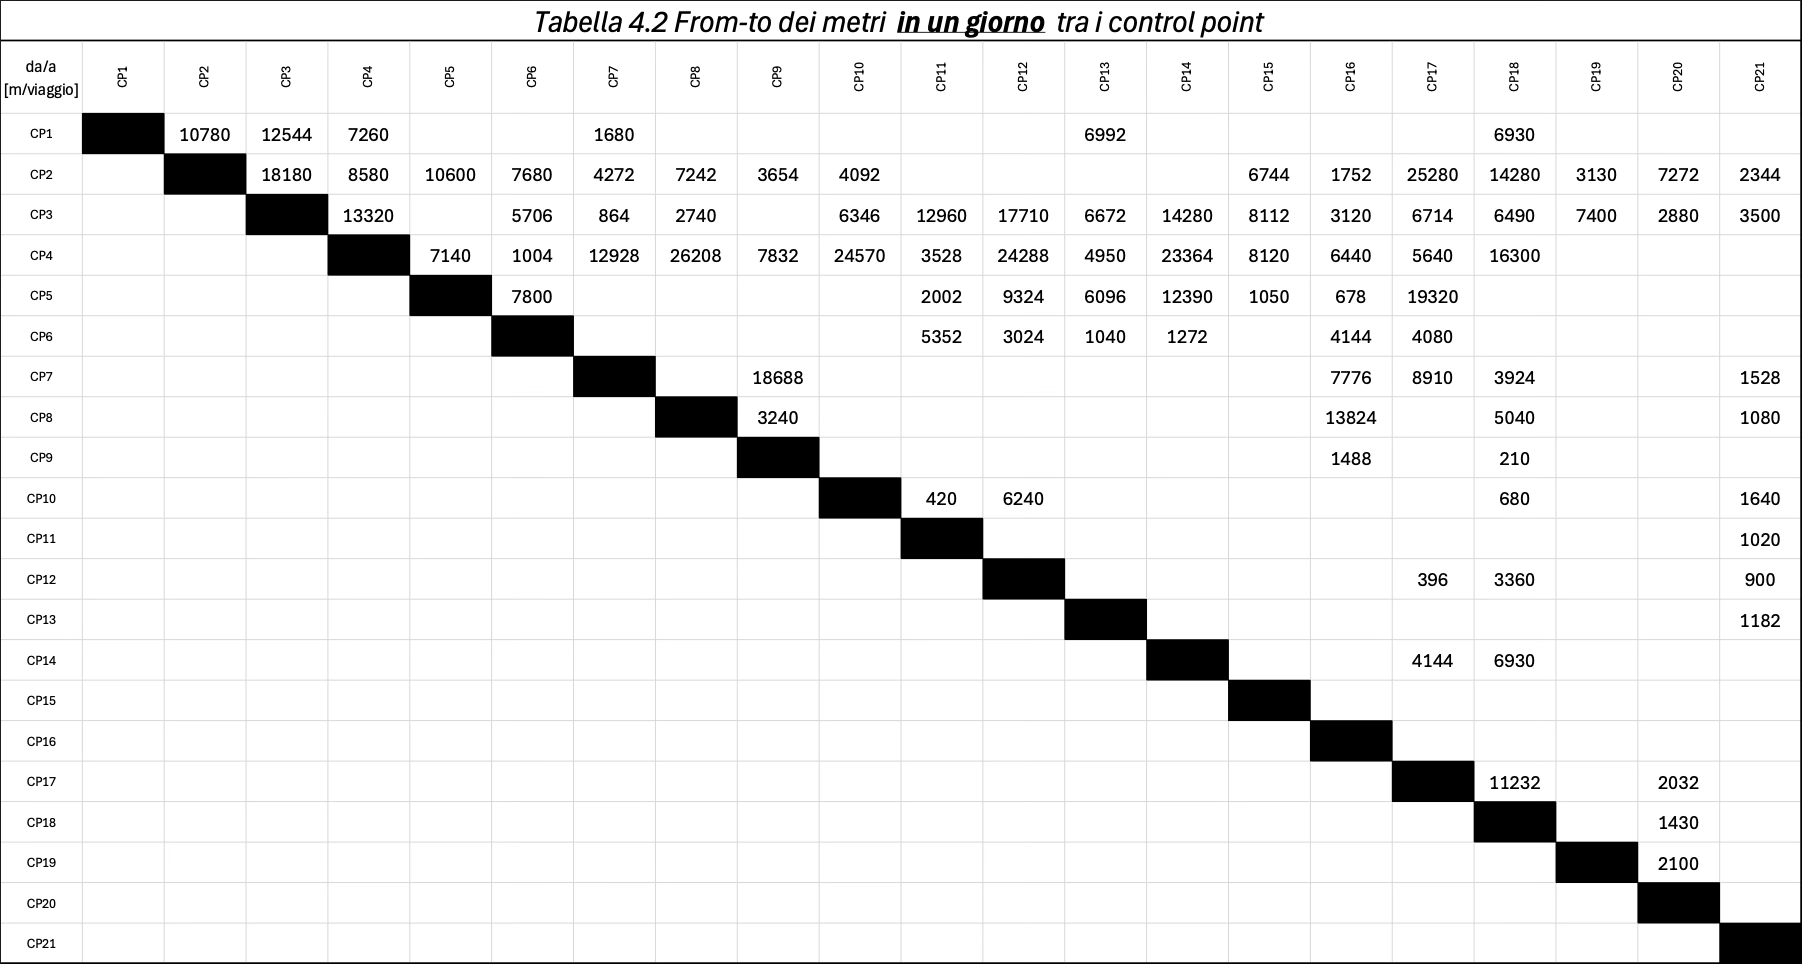
\includegraphics[width=0.7\textwidth]{Tabella 4.2.2.png}
  \caption{From-To dei metri in un giorno tra control point nel caso B}
  \label{fig:From-To dei metri in un giorno tra control point B}
\end{figure}
Il costo di movimentazione globale nel caso B è quindi:
\begin{equation*}
  D_{TOT_{A}} = 649400 \left[\frac{\mathrm{m}}{\mathrm{giorno}}\right]
\end{equation*}
\section{Calcolo del numero di ore mecessarie di operatività delle due tipologie di mezzi ogni giorno}
Dati i seguenti vincoli:

\begin{itemize}
  \item \textbf{Carrelli elevatori}: larghezza minima del corridoio di transito richiesta = 3{,}5~m; velocità media = 2{,}8~m/s; disponibilità media $A = 70\%$.
  \item \textbf{Transpallet}: larghezza minima del corridoio di transito richiesta = 1{,}5~m; velocità media = 0{,}6~m/s; disponibilità media $A = 51\%$.
\end{itemize}

Si osservi che lo stabilimento produttivo comprende più aree dedicate allo stoccaggio. La distanza percorsa dai carrelli elevatori è diversa da quella dei transpallet; la si ottiene confrontando la tabella dei metri percorsi al giorno tra i vari reparti con quella fornita dal testo, che differenzia quale mezzo viene utilizzato per ciascun percorso.

Per calcolare il numero di ore operative giornaliere necessarie per ciascuna tipologia di mezzo, si utilizza la seguente formula:

\begin{equation*}
  \text{hop} = \frac{\text{metri/giorno}}{A \cdot v \cdot 3600}
\end{equation*}

dove:
\begin{itemize}
  \item $\text{metri/giorno}$ = distanza totale percorsa dal mezzo in un giorno,
  \item $A$ = disponibilità media del mezzo,
  \item $v$ = velocità media del mezzo [m/s],
  \item $3600$ = conversione da secondi a ore.
\end{itemize}

Applicando la formula ai dati di ciascun mezzo si ottengono le ore operative giornaliere richieste per carrelli elevatori e transpallet sia nel caso A che nel caso B, specificando per i rispettivi utilizzi. dalle tabelle quì riportate.
In rosso sono indicati gli scambi effettuati con i transpallet, in nero quelli effettuati con i carrelli elevatori.
\begin{figure}[H]
  \centering
  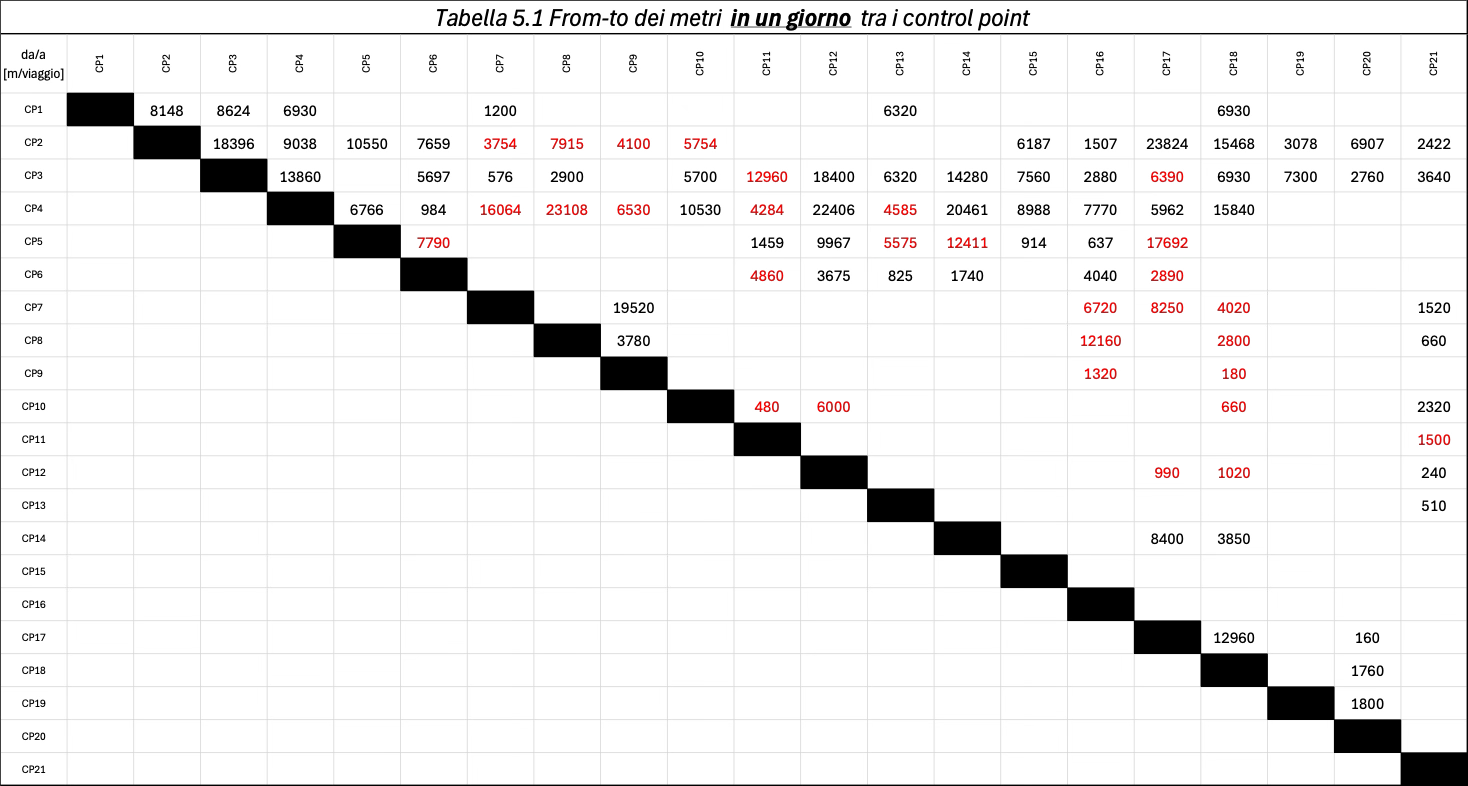
\includegraphics[width=0.8\textwidth]{Tabella 5.1.png}
  \caption{Tabella dei metri percorsi al giorno nel caso A}
  \label{fig:Tabella dei metri percorsi al giorno A}
\end{figure}
\begin{figure}[H]
  \centering
  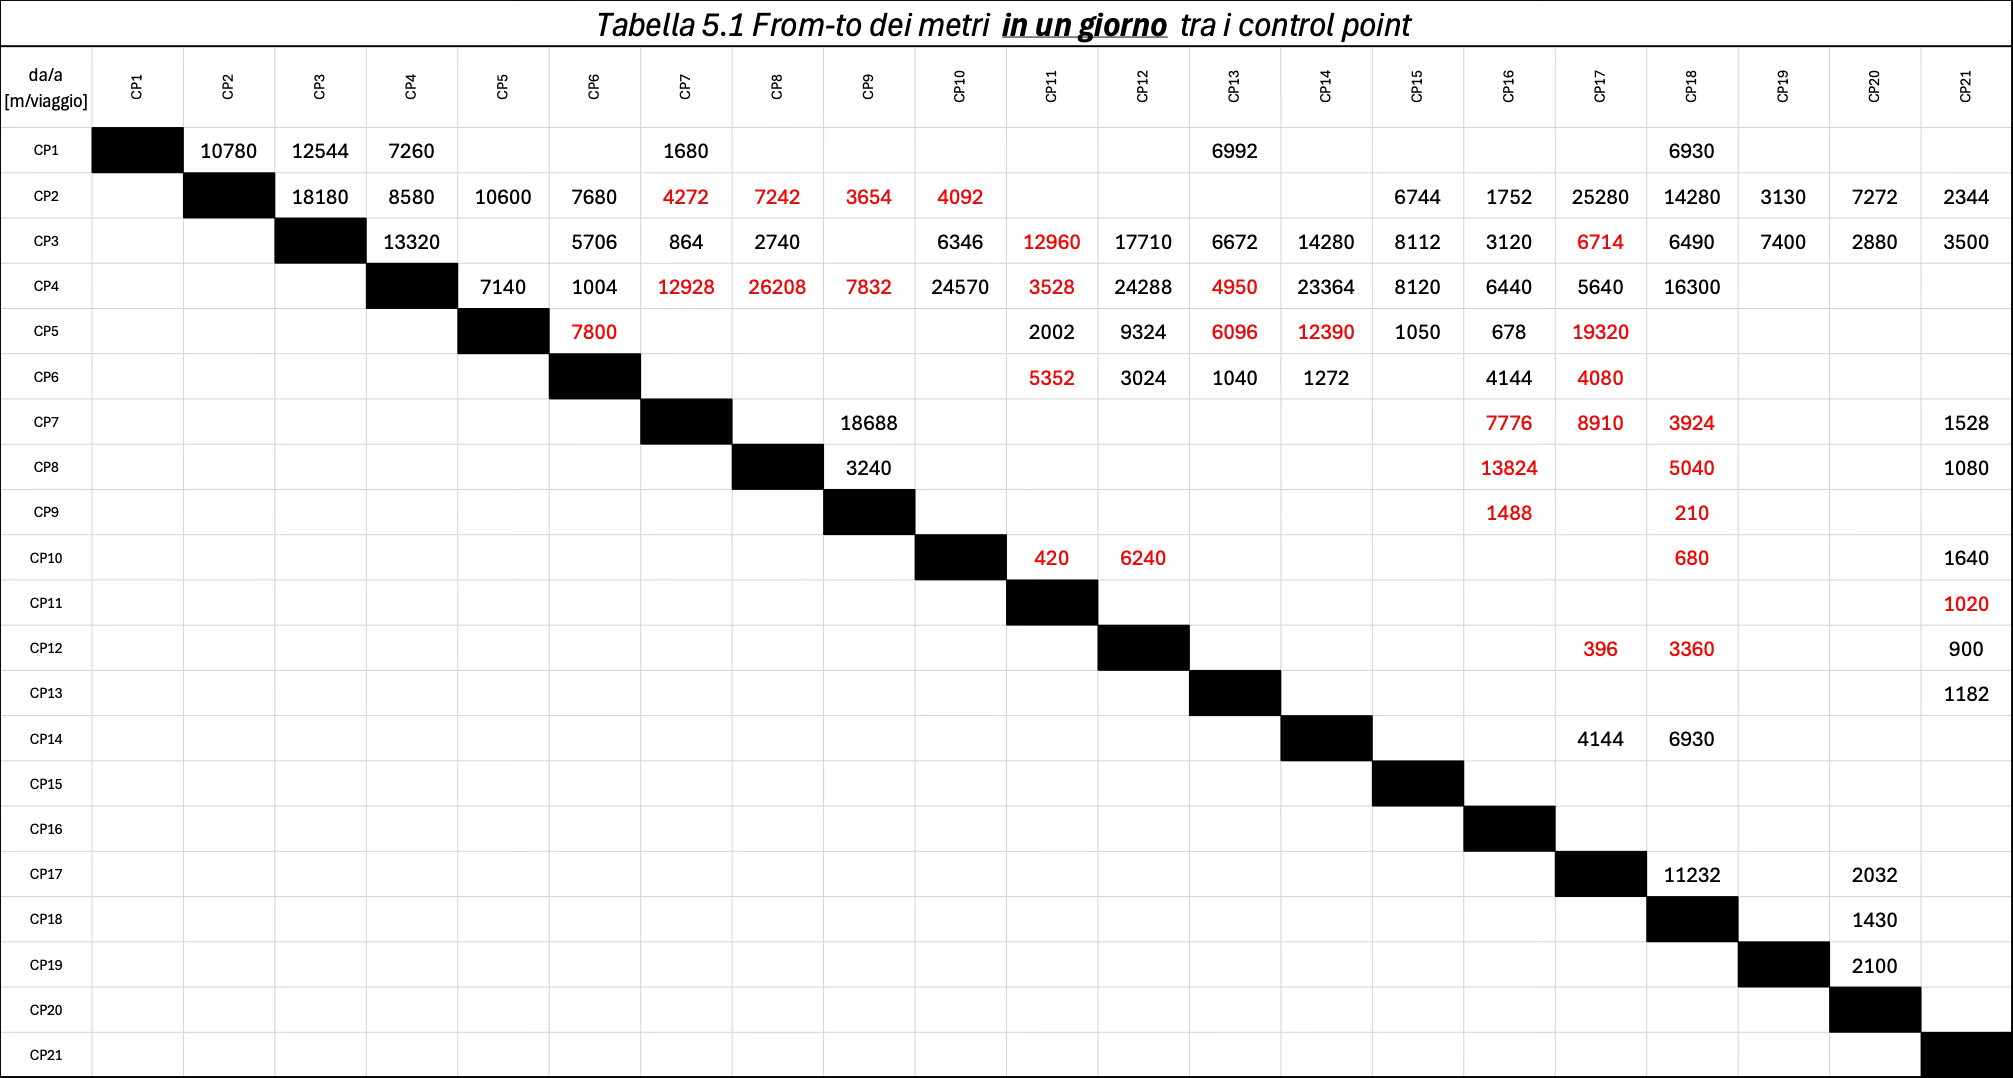
\includegraphics[width=0.8\textwidth]{Tabella 5.2.png}
  \caption{Tabella dei metri percorsi al giorno nel caso B}
  \label{fig:Tabella dei metri percorsi al giorno B}
\end{figure}
\subsection{Carrelli elevatori}
\begin{align*}
  &\text{metri/giorno}_{\text{CE}} = 422433 \left[\frac{\mathrm{m}}{\mathrm{giorno}}\right] \quad \text{(caso A)} \\
  &\text{metri/giorno}_{\text{CE}} = 446694 \left[\frac{\mathrm{m}}{\mathrm{giorno}}\right] \quad \text{(caso B)} \\
  &A_{\text{CE}} = 0.7 \\
  &v_{\text{CE}} = 2.8 \left[\frac{\mathrm{m}}{\mathrm{s}}\right] \\
\end{align*}
\begin{align*}
  &\text{hop}_{\text{CE}} = \frac{\text{metri/giorno}_{\text{CE}}}{A_{\text{CE}} \cdot v_{\text{CE}} \cdot 3600} \\
  &\text{hop}_{\text{CE, A}} = \frac{422433}{0.7 \cdot 2.8 \cdot 3600} \approx 59.86 \left[\mathrm{h}\right] \\
  &\text{hop}_{\text{CE, B}} = \frac{446694}{0.7 \cdot 2.8 \cdot 3600} \approx 63.31 \left[\mathrm{h}\right]
\end{align*}
\subsection{Transpallet}
\begin{align*}
  &\text{metri/giorno}_{\text{TP}} = 192761 \left[\frac{\mathrm{m}}{\mathrm{giorno}}\right] \quad \text{(caso A)} \\
  &\text{metri/giorno}_{\text{TP}} = 202706 \left[\frac{\mathrm{m}}{\mathrm{giorno}}\right] \quad \text{(caso B)} \\
  &A_{\text{TP}} = 0.51 \\
  &v_{\text{TP}} = 0.6 \left[\frac{\mathrm{m}}{\mathrm{s}}\right] \\
\end{align*}
\begin{align*}
  &\text{hop}_{\text{TP}} = \frac{\text{metri/giorno}_{\text{TP}}}{A_{\text{TP}} \cdot v_{\text{TP}} \cdot 3600} \\
  &\text{hop}_{\text{TP, A}} = \frac{192761}{0.51 \cdot 0.6 \cdot 3600} \approx 174.98 \left[\mathrm{h}\right] \\
  &\text{hop}_{\text{TP, B}} = \frac{202706}{0.51 \cdot 0.6 \cdot 3600} \approx 184.01 \left[\mathrm{h}\right]
\end{align*}
\section{Traduzione del costo chilometrico giornaliero in valore economico}
Per tradurre il costo chilometrico giornaliero in valore economico, si adottano i seguenti costi globali di ammortamento ed esercizio: 0{,}043~€/metro per i carrelli elevatori e 0{,}0063~€/metro per i transpallet. Questi valori economici includono sia i costi variabili che quelli fissi associati all’operatività di ciascun mezzo.
Sono stati moltiplicati m/gg per tipologia di mezzo per il loro costo al metro. 
\subsection{Caso A}
\begin{align*}
  &\text{Costo CE} = 422433 \left[\frac{\mathrm{m}}{\mathrm{giorno}}\right] \cdot 0.043 \left[\frac{\text{€}}{\text{m}}\right] \approx 18164.6 \left[\frac{\text{€}}{\mathrm{giorno}}\right] \\
  &\text{Costo TP} = 192761 \left[\frac{\mathrm{m}}{\mathrm{giorno}}\right] \cdot 0.0063 \left[\frac{\text{€}}{\mathrm{m}}\right] \approx 1214.4 \left[\text{€}\right] \\
  &\text{Costo Totale A} = 18144.60 + 1212.99 \approx 19357.59 \left[\text{€}\right]
\end{align*}
\subsection{Caso B}
\begin{align*}
  &\text{Costo CE} = 446694 \left[\frac{\mathrm{m}}{\mathrm{giorno}}\right] \cdot 0.043 \left[\frac{\text{€}}{\text{m}}\right] \approx 19276.02 \left[\frac{\text{€}}{\mathrm{giorno}}\right] \\
  &\text{Costo TP} = 202706 \left[\frac{\mathrm{m}}{\mathrm{giorno}}\right] \cdot 0.0063 \left[\frac{\text{€}}{\text{m}}\right] \approx 1277.45 \left[\text{€}\right] \\
  &\text{Costo Totale B} = 19276.02 + 1277.45 \approx 20553.47 \left[\text{€}\right]
\end{align*}
\section{     Calcolare il numero di carrelli frontali e transpallet necessari e i relativi tassi di utilizzo}
Per calcolare il numero di carrelli frontali e transpallet necessari, si utilizza la seguente formula:
\begin{equation*}
  N = \frac{\text{hop}}{H \cdot R}
\end{equation*}
dove:
\begin{itemize}
  \item $N$ = numero di mezzi necessari,
  \item $\text{hop}$ = ore operative giornaliere richieste,
  \item $H$ = ore lavorative giornaliere disponibili per ciascun mezzo,
  \item $R$ = numero di turni di lavoro giornalieri.
\end{itemize}
\subsection{Carrelli elevatori}
\begin{align*}
  &\text{hop}_{\text{CE, A}} = 59.86 \left[\mathrm{h}\right] \\
  &\text{hop}_{\text{CE, B}} = 63.31 \left[\mathrm{h}\right] \\
  &H_{\text{CE}} = 8 \left[\mathrm{h}\right] \\
  &R_{\text{CE}} = 2 \left[\mathrm{turni}\right] \\
\end{align*}
\begin{align*}
  &N_{\text{CE, A}} = \frac{\text{hop}_{\text{CE, A}}}{H_{\text{CE}} \cdot R_{\text{CE}}} = \frac{59.86}{8 \cdot 2} \approx 3.74 \quad \Rightarrow \quad N_{\text{CE, A}} = 4 \text{ carrelli elevatori} \\
  &N_{\text{CE, B}} = \frac{\text{hop}_{\text{CE, B}}}{H_{\text{CE}} \cdot R_{\text{CE}}} = \frac{63.31}{8 \cdot 2} \approx 3.96 \quad \Rightarrow \quad N_{\text{CE, B}} = 4 \text{carrelli elevatori}
\end{align*}
\subsection{Transpallet}
\begin{align*}
  &\text{hop}_{\text{TP, A}} = 174.98 \left[\mathrm{h}\right] \\
  &\text{hop}_{\text{TP, B}} = 184.01 \left[\mathrm{h}\right] \\
  &H_{\text{TP}} = 8 \left[\mathrm{h}\right] \\
  &R_{\text{TP}} = 2 \left[\mathrm{turni}\right] \\
\end{align*}
\begin{align*}
  &N_{\text{TP, A}} = \frac{\text{hop}_{\text{TP, A}}}{H_{\text{TP}} \cdot R_{\text{TP}}} = \frac{174.98}{8 \cdot 2} \approx 10.93 \quad \Rightarrow \quad N_{\text{TP, A}} = 11 \text{ transpallet} \\
  &N_{\text{TP, B}} = \frac{\text{hop}_{\text{TP, B}}}{H_{\text{TP}} \cdot R_{\text{TP}}} = \frac{184.01}{8 \cdot 2} \approx 11.50 \quad \Rightarrow \quad N_{\text{TP, B}} = 12 \text{ transpallet}
\end{align*}
\subsection{Tassi di utilizzo}
Il tasso di utilizzo di ciascun mezzo è calcolato come:
\begin{equation*}
  U = \frac{\text{hop}}{H \cdot R \cdot N}
\end{equation*}
dove:
\begin{itemize}
  \item $U$ = tasso di utilizzo,
  \item $\text{hop}$ = ore operative giornaliere richieste,
  \item $H$ = ore lavorative giornaliere disponibili per ciascun mezzo,
  \item $R$ = numero di turni di lavoro giornalieri,
  \item $N$ = numero di mezzi necessari.
\end{itemize}
\subsubsection{Carrelli elevatori}
\begin{align*}
  &U_{\text{CE, A}} = \frac{\text{hop}_{\text{CE, A}}}{H_{\text{CE}} \cdot R_{\text{CE}} \cdot N_{\text{CE, A}}} = \frac{59.86}{8 \cdot 2 \cdot 4} \approx 0.93 \quad \Rightarrow \quad U_{\text{CE, A}} = 93\% \\
  &U_{\text{CE, B}} = \frac{\text{hop}_{\text{CE, B}}}{H_{\text{CE}} \cdot R_{\text{CE}} \cdot N_{\text{CE, B}}} = \frac{63.31}{8 \cdot 2 \cdot 4} \approx 0.98 \quad \Rightarrow \quad U_{\text{CE, B}} = 98\%
\end{align*}
\subsubsection{Transpallet}
\begin{align*}
  &U_{\text{TP, A}} = \frac{\text{hop}_{\text{TP, A}}}{H_{\text{TP}} \cdot R_{\text{TP}} \cdot N_{\text{TP, A}}} = \frac{174.98}{8 \cdot 2 \cdot 11} \approx 0.99 \quad \Rightarrow \quad U_{\text{TP, A}} = 99\% \\
  &U_{\text{TP, B}} = \frac{\text{hop}_{\text{TP, B}}}{H_{\text{TP}} \cdot R_{\text{TP}} \cdot N_{\text{TP, B}}} = \frac{184.01}{8 \cdot 2 \cdot 12} \approx 0.96 \quad \Rightarrow \quad U_{\text{TP, B}} = 96\%
\end{align*}
\section{Calcolare il numero di operatori dediti all’attività di movimentazione della merce. Questo è il numero teorico di persone impegnate nel sistema a tempo pieno nella movimentazione della merce.}
Per quanto riguarda il numero di operai è stato diviso il numero di ore di operatività per le ore di ciascun turno.
\subsection{Carrelli elevatori}
\begin{align*}
  &\text{hop}_{\text{CE, A}} = 59.86 \left[\mathrm{h}\right] \\
  &\text{hop}_{\text{CE, B}} = 63.31 \left[\mathrm{h}\right] \\
  &H_{\text{CE}} = 8 \left[\mathrm{h}\right] \\
\end{align*}
\begin{align*}
  &N_{\text{operai, CE, A}} = \frac{\text{hop}_{\text{CE, A}}}{H_{\text{CE}}} = \frac{59.86}{8} \approx 7.48 \quad \Rightarrow \quad N_{\text{operai, CE, A}} = 8 \text{ operai} \\
  &N_{\text{operai, CE, B}} = \frac{\text{hop}_{\text{CE, B}}}{H_{\text{CE}}} = \frac{63.31}{8} \approx 7.91 \quad \Rightarrow \quad N_{\text{operai, CE, B}} = 8 \text{ operai}
\end{align*}
\subsection{Transpallet}
\begin{align*}
  &\text{hop}_{\text{TP, A}} = 174.98 \left[\mathrm{h}\right] \\
  &\text{hop}_{\text{TP, B}} = 184.01 \left[\mathrm{h}\right] \\
  &H_{\text{TP}} = 8 \left[\mathrm{h}\right] \\
\end{align*}
\begin{align*}
  &N_{\text{operai, TP, A}} = \frac{\text{hop}_{\text{TP, A}}}{H_{\text{TP}}} = \frac{174.98}{8} \approx 21.87 \quad \Rightarrow \quad N_{\text{operai, TP, A}} = 22 \text{ operai} \\
  &N_{\text{operai, TP, B}} = \frac{\text{hop}_{\text{TP, B}}}{H_{\text{TP}}} = \frac{184.01}{8} \approx 23.00 \quad \Rightarrow \quad N_{\text{operai, TP, B}} = 23 \text{ operai}
\end{align*}
\section{ Calcolare il costo della manodopera dedicata alla movimentazione/logistica, sapendo quello unitario lordo è pari a 30 €/(h x operaio).}
Conoscendo il costo orario (30 €/h*operaio) è stata moltiplicata tale cifra per il numero di operatori coinvolti nella movimentazione/logistica.
\subsection{Carrelli elevatori}
\begin{align*}
  &\text{costo orario}_{\text{CE}} = 30 \left[\frac{\text{€}}{\mathrm{h} \cdot \text{operaio}}\right] \\
  &\text{costo giornaliero}_{\text{CE, A}} = N_{\text{operai, CE, A}} \cdot H \cdot \text{costo orario}_{\text{CE}} = 8 \cdot 8 \cdot 30 \approx 1920\left[\text{€}\right] \\
  &\text{costo giornaliero}_{\text{CE, B}} = N_{\text{operai, CE, B}} \cdot H \cdot \text{costo orario}_{\text{CE}} = 8 \cdot 8 \cdot 30 \approx 1920 \left[\text{€}\right]
\end{align*}
\subsection{Transpallet}
\begin{align*}
  &\text{costo orario}_{\text{TP}} = 30 \left[\frac{\text{€}}{\mathrm{h} \cdot \text{operaio}}\right] \\
  &\text{costo giornaliero}_{\text{TP, A}} = N_{\text{operai, TP, A}} \cdot H \cdot \text{costo orario}_{\text{TP}} = 22 \cdot 8 \cdot 30 \approx 5280 \left[\text{€}\right] \\
  &\text{costo giornaliero}_{\text{TP, B}} = N_{\text{operai, TP, B}} \cdot H \cdot \text{costo orario}_{\text{TP}} = 23 \cdot 8 \cdot 30 \approx 5520 \left[\text{€}\right]
\end{align*}
\end{document}


